%=============================================================================
%  TalentPulse -- Comprehensive Capstone Report (Modules 1, 2, 3)
%  CSE 450, Department of CSE, Bangladesh University of Engineering and Technology
%  Compile with pdflatex (run twice for TOC/references)
%=============================================================================
\documentclass[11pt,a4paper]{article}

%------------------------------------------------ core packages
\usepackage[a4paper,top=2.4cm,bottom=2.6cm,left=2.4cm,right=2.4cm,headsep=12pt]{geometry}
\usepackage[utf8]{inputenc}
\usepackage[T1]{fontenc}
\usepackage{lmodern}
\usepackage[scaled=0.92]{helvet}
\usepackage{microtype}
\usepackage{amsmath,amssymb}
\usepackage{booktabs}
\usepackage{array}
\usepackage{longtable}
\usepackage{colortbl}
\usepackage{graphicx}
\usepackage{tikz}
\usetikzlibrary{arrows.meta,positioning,shapes.geometric,calc,fit,backgrounds,decorations.pathreplacing}
\usepackage{enumitem}
\usepackage{titlesec}
\usepackage{fancyhdr}
\usepackage{caption}
\usepackage{float}
\usepackage{tabularx}
\usepackage{multirow}
\usepackage{pifont}
\usepackage[hidelinks]{hyperref}
\usepackage{bookmark}

%------------------------------------------------ palette (shared with the project's presentation deck)
\definecolor{TPnavy}{RGB}{15,52,80}
\definecolor{TPteal}{RGB}{18,110,120}
\definecolor{TPgold}{RGB}{193,138,52}
\definecolor{TPgreen}{RGB}{40,120,86}
\definecolor{TPred}{RGB}{176,58,58}
\definecolor{TPbg}{RGB}{252,251,248}
\definecolor{TPgray}{RGB}{92,100,108}
\definecolor{TPlight}{RGB}{234,240,240}
\definecolor{TPlightgold}{RGB}{247,241,229}

% dedicated, more vibrant heading colours -- deliberately darker and more
% saturated than the TPnavy/TPteal/TPgold used for boxes and rules, so
% headings read clearly against both body text and each other
\definecolor{HeadOne}{RGB}{86,22,125}
\definecolor{HeadTwo}{RGB}{0,102,94}
\definecolor{HeadThree}{RGB}{168,84,0}

%------------------------------------------------ section heading style
\titleformat{\section}
  {\normalfont\Large\bfseries\color{HeadOne}}
  {\thesection}{0.6em}{}
  [{\color{TPteal}\titlerule[1.1pt]}]
\titleformat{\subsection}
  {\normalfont\large\bfseries\color{HeadTwo}}
  {\thesubsection}{0.6em}{}
\titleformat{\subsubsection}
  {\normalfont\normalsize\bfseries\color{HeadThree}}
  {\thesubsubsection}{0.6em}{}
\titlespacing*{\section}{0pt}{1.6em}{0.9em}
\titlespacing*{\subsection}{0pt}{1.2em}{0.6em}
\titlespacing*{\subsubsection}{0pt}{1.0em}{0.4em}

%------------------------------------------------ header / footer
\pagestyle{fancy}
\fancyhf{}
\renewcommand{\headrulewidth}{0.6pt}
\renewcommand{\footrulewidth}{0.4pt}
\fancyhead[L]{\small\color{TPgray}\textit{TalentPulse}}
\fancyhead[R]{\small\color{TPgray}\leftmark}
\fancyfoot[L]{\small\color{TPgray}CSE 450 Capstone Project}
\fancyfoot[R]{\small\color{TPnavy}\thepage}
\renewcommand{\headrule}{\color{TPteal}\hrule height\headrulewidth}
\renewcommand{\sectionmark}[1]{\markboth{#1}{}}

\fancypagestyle{plain}{%
  \fancyhf{}
  \fancyfoot[L]{\small\color{TPgray}CSE 450 Capstone Project}
  \fancyfoot[R]{\small\color{TPnavy}\thepage}
  \renewcommand{\headrulewidth}{0pt}
}

%------------------------------------------------ hyperref colours
\hypersetup{
  colorlinks=true,
  linkcolor=HeadTwo,
  citecolor=HeadTwo,
  urlcolor=HeadTwo,
  pdftitle={TalentPulse -- Intelligent Employee Management System},
  pdfauthor={Anuron Maitro, Md. Asif Ali, Md. Maruf Hasan Rubab, Himadri Gobinda Biswas, Md. Rafat Kabir},
  pdfsubject={CSE 450 Capstone Project Report},
  bookmarksopen=true,
  bookmarksdepth=3
}

%------------------------------------------------ caption style
\captionsetup{font={small,color=TPgray},labelfont={bf,color=TPnavy},labelsep=colon,margin=1cm}

%------------------------------------------------ small helper macros
\newcommand{\gd}[1]{{\color{TPgreen}\bfseries #1}}
\newcommand{\bd}[1]{{\color{TPred}\bfseries #1}}
\newcommand{\hdrow}{\rowcolor{TPnavy}}
\newcommand{\hdtxt}[1]{\textcolor{white}{\bfseries #1}}
\newcommand{\code}[1]{\texttt{\footnotesize #1}}

% shared TikZ node styles for pipeline diagrams across the report
\tikzset{
  stage/.style={rounded corners=3pt,draw=TPteal,line width=1pt,fill=TPlight,
                text=TPnavy,align=center,inner sep=6pt,font=\footnotesize\bfseries,
                minimum height=1.05cm,text width=2.35cm},
  data/.style={rounded corners=3pt,draw=TPgold,line width=1pt,fill=TPlightgold,
               text=TPnavy,align=center,inner sep=6pt,font=\footnotesize,
               minimum height=1.05cm,text width=2.35cm},
  decision/.style={diamond,draw=TPred,line width=1pt,fill=TPred!8,
               text=TPnavy,align=center,inner sep=3pt,font=\scriptsize,
               aspect=2.2},
  fl/.style={-{Stealth[length=2.4mm]},line width=1.05pt,draw=TPteal},
  flg/.style={-{Stealth[length=2.4mm]},line width=1.05pt,draw=TPgold},
  flr/.style={-{Stealth[length=2.4mm]},line width=1.05pt,draw=TPred},
  note/.style={font=\scriptsize,text=TPgray,align=left}
}

% consistent formula panel: a thin rule above and below the formula.
% Deliberately NOT a tabular or an \fbox-split-across-braces trick, since
% both interfere with \\ inside align/cases environments placed inside it.
\newenvironment{formulabox}
  {\begin{center}\color{TPteal}\rule{0.92\linewidth}{0.8pt}\par\vspace{5pt}\color{TPnavy}}
  {\par\vspace{3pt}\color{TPteal}\rule{0.92\linewidth}{0.8pt}\end{center}}

\renewcommand{\arraystretch}{1.15}
\newcolumntype{C}[1]{>{\centering\arraybackslash}p{#1}}

%=============================================================================
\begin{document}
\raggedbottom

%============================================================================
% TITLE PAGE
%============================================================================
\begin{titlepage}
\pagestyle{empty}
\begin{center}

\vspace*{0.3cm}
\includegraphics[width=2.5cm]{images/buet-logo.png}

\vspace{0.4cm}
{\large\bfseries Department of Computer Science and Engineering}\\[0.1cm]
{\large\bfseries Bangladesh University of Engineering and Technology}\\[0.1cm]
{\normalsize Dhaka, Bangladesh}

\vspace{0.8cm}
{\Huge\bfseries TalentPulse}\\[0.3cm]
{\Large\bfseries An Intelligent Employee Management System}

\vspace{0.6cm}
{\color{black!40}\rule{0.65\linewidth}{0.6pt}}

\vspace{0.6cm}
{\large\bfseries Project Implementation Report}\\[0.2cm]
%{\normalsize Submitted in partial fulfillment of the requirements for the course}\\[0.1cm]
{\normalsize\bfseries CSE 450: Capstone Project}

\vspace{0.8cm}
{\bfseries\large Submitted by}\\[0.25cm]
\begin{tabular}{p{6.8cm} c}
\toprule
\textbf{Student Name} & \textbf{Student ID} \\
\midrule
Anuron Maitro & 2105037 \\
Md.\ Asif Ali & 2105038 \\
Md.\ Maruf Hasan Rubab & 2105042 \\
Himadri Gobinda Biswas & 2105047 \\
Md.\ Rafat Kabir & 2105054 \\
\bottomrule
\end{tabular}

\vspace{0.7cm}
\begin{tabular}{ll}
\textbf{Supervisor:} & \textbf{Dr.\ Sadia Sharmin} \\
& Professor, Department of CSE, BUET \\[0.25cm]
\textbf{Industry Mentors:} & \textbf{Ahsanul Ameen Sabit}, \textbf{M.\ Ebrahim Sazin} \\
& IQVIA \\
\end{tabular}

\vfill
{\normalsize Section A2 \quad $\cdot$ \quad Group 03}\\[0.2cm]
{\normalsize\bfseries September 2026}

\vspace*{0.2cm}
\end{center}
\end{titlepage}

\clearpage
\pagestyle{fancy}
\pagenumbering{roman}

%============================================================================
\tableofcontents
\clearpage
\listoffigures
\clearpage
\listoftables
\clearpage
\pagenumbering{arabic}
\setcounter{page}{1}

%============================================================================
\section{Introduction}
\label{sec:intro}

This section introduces TalentPulse, outlining the foundational challenges across the enterprise employee lifecycle, the scope and core objectives of the project, and the structural organization of this capstone report.

\subsection{Overview of TalentPulse}

TalentPulse is an AI-driven human resource management system built to bring three otherwise disconnected stages of the employee lifecycle, namely hiring, growth, and retention, under one coherent, data-driven platform. Traditional HR management systems provide record-keeping, workflow automation, and basic reporting, but they generally stop short of decision support. A recruiter is still left to read a stack of resumes by eye, an HR manager rarely has a systematic way to plan a specific employee's next training step, and attrition is usually discovered only after a resignation letter has already been submitted. TalentPulse was designed specifically to close these three gaps with purpose-built machine learning components rather than generic dashboards.

The system is organized into three cooperating modules, each addressing one stage of that lifecycle:

\begin{enumerate}[label=\textbf{Module \arabic*.}, leftmargin=2.6cm]
  \item \textbf{Fairness-Aware Resume Screening and Skill Extraction.} A fine-tuned Sentence-BERT encoder ranks candidates against a job description by semantic similarity rather than keyword overlap, and an adversarially trained companion model strips demographic signal, specifically gender, university tier, skin colour, and ethnicity, out of that ranking, so that the score reflects skill rather than identity.
  \item \textbf{Intelligent Skill-Gap Analysis and Learning Path Recommendation.} A zero-shot named-entity extractor reads real skills out of free-text resumes and job descriptions, a semantic gap-analysis engine measures how far an employee's current skill profile sits from a target role, and a constrained course-recommendation algorithm assembles an ordered, budget-aware learning path to close that gap.
  \item \textbf{Explainable Employee Attrition Prediction.} A two-stage ensemble of gradient-boosted trees first estimates the probability that a given employee will leave, and a second classifier proposes the most likely underlying reason. SHAP values explain each individual prediction in terms of the specific features driving it, and a counterfactual engine proposes the smallest realistic change to an employee's situation that would measurably reduce their risk.
\end{enumerate}

These three modules are not independent demonstrations bolted together for a presentation; they share one MongoDB-backed application, one role-based identity model, and one continuous employee record that moves from applicant, to hire, to tracked employee, to (where relevant) an alumnus with a documented departure reason. Section~\ref{sec:frontend} of this report walks through that shared application in full, using the same worked examples that were used to verify it against the live, deployed system rather than against source code alone.

\subsection{Problem Statement}

Three concrete, independent problems motivated this project, and each maps directly onto one module:

\begin{itemize}[leftmargin=1.4cm]
  \item \textbf{Hiring is inconsistent and can be demonstrably biased.} Manual and even automated resume screening can reward candidates for attributes that have no bearing on their actual competence, such as the prestige of their university or demographic markers implicit in their name or background. Left unchecked, an AI system trained on historical hiring data can silently reproduce and amplify exactly this kind of bias rather than removing it.
  \item \textbf{Employee upskilling is rarely planned, and almost never budgeted.} When a skill gap is identified, the typical response is a vague instruction (``you should learn Docker'') with no structured plan for how long that will realistically take, what it will cost, or in what order prerequisite material should be studied.
  \item \textbf{Attrition is detected reactively, not proactively.} Most organizations learn that an employee is unhappy only when they resign. There is rarely a systematic, per-employee estimate of departure risk, an explanation of what is actually driving that risk, or a concrete, costed intervention plan that could change the outcome before it happens.
\end{itemize}

\subsection{Project Scope and Objectives}

The scope of TalentPulse, as actually implemented and verified end to end against the running system, is as follows:

\begin{itemize}[leftmargin=1.4cm]
  \item Build and fine-tune a resume-to-job-description matching model, and train a bias-mitigation companion model on top of it, both trained on purpose-built datasets described in Section~\ref{sec:mod1}.
  \item Build a skill-extraction, gap-analysis, and course-recommendation pipeline that operates on real, uploaded resumes and job postings, described in Section~\ref{sec:mod2}.
  \item Build a two-stage attrition classifier with per-employee explainability and actionable counterfactual interventions, described in Section~\ref{sec:mod3}.
  \item Integrate all three modules behind one production web application with authenticated, role-based access for HR administrators, employees, and job applicants, described in Section~\ref{sec:frontend}.
  \item Deploy every model as an independently hosted inference service so that the heavy machine-learning workloads never block the everyday application traffic, described in Section~\ref{sec:techstack}.
\end{itemize}

The system deliberately targets small-to-medium enterprises, with particular consideration for the Bangladeshi market, where equivalent commercial HR intelligence tooling is either unavailable or priced far outside what such an organization can justify. This positioning, and the specific products TalentPulse was built in response to, is developed in full in Section~\ref{sec:motivation}.

\subsection{Report Organization}

The remainder of this report is organized as follows. Section~\ref{sec:motivation} places TalentPulse against existing commercial HR software and explains the specific gap each module was built to close. Section~\ref{sec:arch} gives a system-wide architectural overview, including how the system's design evolved over the course of the project. Sections~\ref{sec:mod1}, \ref{sec:mod2}, and \ref{sec:mod3} form the technical core of the report, covering every dataset, model, formula, and design decision behind each module in full detail, with an accompanying pipeline diagram for each. Section~\ref{sec:techstack} documents the technology stack and deployment topology as they exist in the live system. Section~\ref{sec:frontend} narrates the complete end-user workflow across every screen of the application. Section~\ref{sec:screenshots} reserves ten full pages for annotated screenshots of the running application. Section~\ref{sec:discussion} discusses the project's strengths and honest limitations, and Section~\ref{sec:conclusion} concludes the report.

\clearpage
%============================================================================
\section{Motivation and Related Work}
\label{sec:motivation}

This section examines the current commercial HR software landscape, positions TalentPulse against established enterprise solutions, and details the specific accessibility, fairness, and retention gaps that motivated each module.

\subsection{The State of Commercial HR Technology}

Software that performs some version of what each TalentPulse module does already exists commercially, and it is important to be precise about that rather than to claim the field is empty. What distinguishes TalentPulse is not that the underlying problem is unaddressed, but that the existing solutions are priced, packaged, and positioned in ways that leave a specific and substantial market segment unserved: organizations, particularly in markets such as Bangladesh, that need this class of tooling but cannot justify an enterprise software contract to obtain it.

Three categories of established product map onto the three TalentPulse modules, summarized in Table~\ref{tab:competitors}.

\begin{table}[H]
\centering
\caption{Representative commercial products by category, and their positioning relative to TalentPulse}
\label{tab:competitors}
\small
\begin{tabular}{p{3.0cm}p{4.6cm}p{7.0cm}}
\toprule
\hdrow \hdtxt{Category} & \hdtxt{Representative products} & \hdtxt{Typical positioning} \\
\midrule
Hiring \& screening & HireVue, Eightfold AI, Workday Recruiting & Enterprise applicant-tracking and AI-screening suites, typically sold on multi-year contracts to organizations with dedicated recruiting operations. \\
\rowcolor{TPlight}
Skilling \& growth & Degreed, Cornerstone, Gloat & Learning-experience and internal talent-marketplace platforms, generally licensed per employee seat at enterprise volume. \\
Retention \& analytics & Culture Amp, Workday Peakon, Workhuman & Engagement-survey and recognition platforms that measure sentiment in aggregate, rather than predicting individual departure risk. \\
\bottomrule
\end{tabular}
\end{table}

\subsection{Module 1: The Cost and the Bias Problem in Automated Screening}
The cost structure of modern applicant-tracking systems (ATS) with embedded AI screening, such as Eightfold AI or HireVue, reflects an enterprise sales model: multi-year contracts, implementation fees running into tens of thousands of dollars, and minimum seat counts designed for large human-resource departments. For a mid-sized technology firm in Dhaka or Chittagong hiring twenty to fifty engineers per year, such software is economically inaccessible. The default alternative remains manual screening, which is slow, inconsistent, and highly prone to unconscious bias.

Commercial screening tools that do incorporate machine learning have repeatedly demonstrated a second, more dangerous failure mode: automating and amplifying historical human bias rather than removing it. When an AI model is trained on past hiring decisions, it learns to treat the demographic characteristics of previously hired candidates, such as attendance at a prestigious national university, gender, or community background, as positive predictive features, effectively laundering bias through an opaque algorithm. The high-profile class-action certification in \textit{Mobley v.\ Workday, Inc.} (2025), alleging algorithmic discrimination across protected demographic classes in automated applicant screening, underscores that this is not an abstract academic concern but an active legal and operational risk in deployed commercial software.

Module 1 was designed from the outset with both problems in mind. It is delivered as an accessible, self-hostable service requiring no enterprise contract, and its architecture couples semantic ranking with explicit, adversarial bias mitigation across four protected demographic factors (gender, university tier, skin colour, and ethnicity), so that candidates are ranked by what they can do rather than where they come from.

\subsection{Module 2: The Access Gap in Structured Upskilling}

Learning-experience and talent-marketplace platforms in the Degreed, Cornerstone, and Gloat category are almost universally sold through enterprise procurement, with published estimates commonly placing custom enterprise pricing at \$100{,}000 or more annually once a deployment covers a meaningful employee base. The practical consequence is an access gap rather than a capability gap: the underlying idea of matching an employee's skill profile against a target role and recommending a structured course of study is well understood, but the tooling that does it automatically is reserved for organizations that can already afford a dedicated learning-and-development budget. Everyone else is left to work out what to learn next largely unaided. Module 2 was built to deliver the same category of capability, skill extraction, quantified gap analysis, and a budget-and-time-constrained course plan, without that licensing barrier.

\subsection{Module 3: The Detection Gap in Retention Tooling}

Culture Amp, Workday Peakon, and Workhuman are all genuinely useful, and genuinely different in kind from what Module 3 does. Culture Amp and Peakon are principally engagement-survey platforms: they ask employees how they feel, in aggregate, on a recurring cadence, and surface sentiment trends after the fact. Workhuman is principally a peer-recognition and rewards platform. None of the three, as core functionality, produces a quantified, individual-level probability that a specific named employee will leave within a defined horizon, explains that probability in terms of the actual features driving it for that person, or proposes a specific, ranked set of interventions together with their predicted effect on that individual's risk score before any survey has even been sent. That is the specific capability Module 3 was built to provide, and Section~\ref{sec:mod3} documents its accuracy, its explainability layer, and its intervention engine in full.

\subsection{Summary of Contribution}

TalentPulse's contribution is not a single novel algorithm; it is the integration of three purpose-built, individually rigorous machine learning pipelines, resume-JD semantic matching with adversarial debiasing, skill-gap-aware learning path recommendation, and explainable attrition prediction with counterfactual interventions, behind one connected, low-cost application, verified end to end against a real deployed system rather than described only in the abstract. Every claim made about accuracy, fairness improvement, or system behaviour in the remainder of this report is drawn from an actual measured result, a real dataset statistic, or a behaviour directly observed in the running application, and is presented as such.

\clearpage
%============================================================================
\section{System Architecture}
\label{sec:arch}

This section describes the end-to-end system architecture of TalentPulse, tracing the evolution from the initial four-tier conceptual blueprint to the deployed decoupled microservices infrastructure.

\subsection{Architectural Evolution}

TalentPulse's architecture was not fixed at the start of the project; it evolved through a formal system-analysis-and-design phase into the architecture that was actually built and deployed. This evolution is documented here deliberately, because it reflects genuine engineering decisions rather than an oversight. The project's original System Analysis and Design report specified a four-layer architecture with polyglot persistence: a React and Tailwind CSS presentation layer, a dual-service application layer combining Node.js/Express (application logic and authentication) with a separate FastAPI bridge (ML inference), and a data layer split between PostgreSQL (structured HR records) and MongoDB (flexible, JSON-shaped ML outputs). Figure~\ref{fig:arch-original} reproduces the intent of that original four-layer plan.

\begin{figure}[H]
\centering
\resizebox{\linewidth}{!}{%
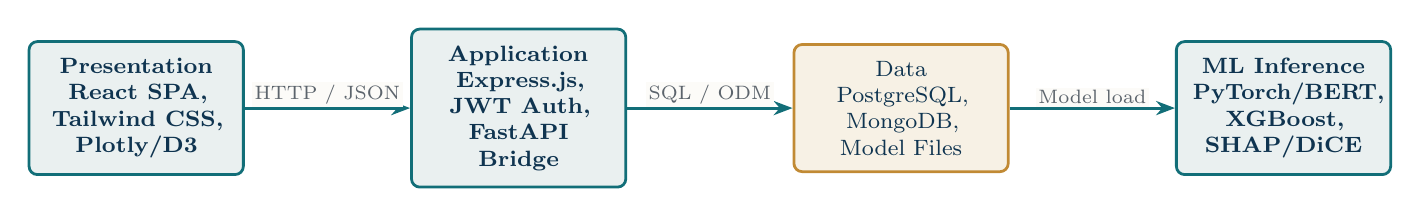
\begin{tikzpicture}[node distance=2.1cm]
  \node[stage,text width=2.3cm,fill=TPlight] (pres) {Presentation\\\footnotesize React SPA, Tailwind CSS, Plotly/D3};
  \node[stage,text width=2.3cm,right=of pres] (app) {Application\\\footnotesize Express.js, JWT Auth, FastAPI Bridge};
  \node[data,text width=2.3cm,right=of app,fill=TPlightgold,draw=TPgold] (data) {Data\\\footnotesize PostgreSQL, MongoDB, Model Files};
  \node[stage,text width=2.3cm,right=of data,fill=TPlight] (ml) {ML Inference\\\footnotesize PyTorch/BERT, XGBoost, SHAP/DiCE};
  \draw[fl] (pres) -- node[above,note,fill=TPbg,inner sep=1pt]{HTTP / JSON} (app);
  \draw[fl] (app) -- node[above,note,fill=TPbg,inner sep=1pt]{SQL / ODM} (data);
  \draw[fl] (data) -- node[above,note,fill=TPbg,inner sep=1pt]{Model load} (ml);
\end{tikzpicture}}
\caption{The originally planned four-layer architecture with polyglot (PostgreSQL + MongoDB) persistence, as specified in the project's initial System Analysis and Design phase.}
\label{fig:arch-original}
\end{figure}

As development progressed, this plan was deliberately simplified. The dedicated PostgreSQL layer was consolidated into MongoDB alone, since the project's actual data, resumes, applications, screening runs, and learning paths, is naturally document-shaped and benefits more from MongoDB's flexible schema than from a fixed relational schema designed around the IBM HR Analytics dataset's column layout. The single FastAPI bridge was split into three independently deployed FastAPI services, one per module (with Module 1 further split into a skill-extraction service and a ranking/debiasing service), each hosted as its own container on Hugging Face Spaces, rather than one bridge process handling all inference. This is the architecture that was actually built, deployed, and verified, and it is the architecture documented for the remainder of this report.

\clearpage
\subsection{Final Deployed Architecture}

The deployed system separates concerns into three tiers, illustrated in Figure~\ref{fig:arch-final}: a React single-page application; an Express.js backend that owns authentication, business logic, and the single MongoDB database; and four independently hosted Python inference services, one for skill extraction, one for resume-JD ranking and debiasing, one for skill-gap analysis and course recommendation, and one for attrition prediction. The browser never calls an inference service directly; every ML call is proxied through the Express backend, which keeps a single authentication and authorization boundary in front of every capability in the system.

\begin{figure}[H]
\centering
\resizebox{\linewidth}{!}{%
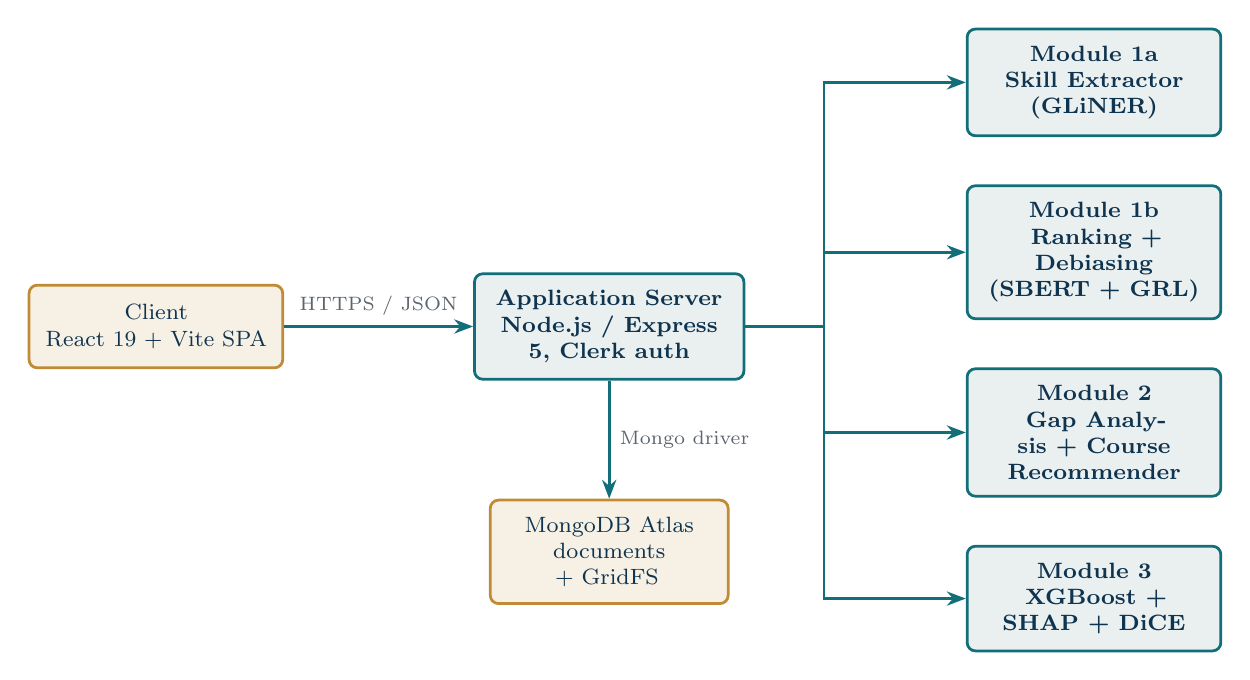
\begin{tikzpicture}[node distance=1.05cm]
  \node[data,text width=2.8cm,fill=TPlightgold,draw=TPgold] (client) {Client\\\footnotesize React 19 + Vite SPA};
  \node[stage,text width=3.0cm,right=2.4cm of client] (express) {Application Server\\\footnotesize Node.js / Express 5, Clerk auth};
  \node[data,text width=2.6cm,below=1.5cm of express,fill=TPlightgold,draw=TPgold] (mongo) {MongoDB Atlas\\\footnotesize documents + GridFS};

  \node[stage,text width=2.8cm,right=2.8cm of express,yshift=3.1cm,fill=TPlight] (m1a) {Module 1a\\\footnotesize Skill Extractor (GLiNER)};
  \node[stage,text width=2.8cm,below=0.6cm of m1a,fill=TPlight] (m1b) {Module 1b\\\footnotesize Ranking + Debiasing (SBERT + GRL)};
  \node[stage,text width=2.8cm,below=0.6cm of m1b,fill=TPlight] (m2) {Module 2\\\footnotesize Gap Analysis + Course Recommender};
  \node[stage,text width=2.8cm,below=0.6cm of m2,fill=TPlight] (m3) {Module 3\\\footnotesize XGBoost + SHAP + DiCE};

  \draw[fl] (client) -- node[above,note]{HTTPS / JSON} (express);
  \draw[fl] (express) -- node[right,note]{Mongo driver} (mongo);
  \draw[fl] (express.east) -- ($(express.east)+(1.0,0)$) |- (m1a.west);
  \draw[fl] (express.east) -- ($(express.east)+(1.0,0)$) |- (m1b.west);
  \draw[fl] (express.east) -- ($(express.east)+(1.0,0)$) |- (m2.west);
  \draw[fl] (express.east) -- ($(express.east)+(1.0,0)$) |- (m3.west);
\end{tikzpicture}}
\caption{The final, deployed TalentPulse architecture. All four ML services are independently hosted FastAPI containers on Hugging Face Spaces, called exclusively through the Express backend.}
\label{fig:arch-final}
\end{figure}

\subsection{Deployment Topology}

Table~\ref{tab:deploy} lists where each component of the running system actually lives.

\begin{table}[H]
\centering
\caption{Deployment topology of the live TalentPulse system}
\label{tab:deploy}
\small
\begin{tabular}{p{3.2cm}p{5.8cm}p{5.4cm}}
\toprule
\hdrow \hdtxt{Component} & \hdtxt{Technology} & \hdtxt{Hosting} \\
\midrule
Frontend & React 19, Vite, Tailwind CSS & Vercel \\
\rowcolor{TPlight}
Backend API & Node.js, Express 5 & Vercel serverless functions \\
Database & MongoDB Atlas & Cloud-hosted, document store + GridFS for CV files \\
\rowcolor{TPlight}
Authentication & Clerk & Role-based sessions: applicant, employee, admin \\
Module 1 -- skill extractor & Python, GLiNER, FastAPI & Hugging Face Spaces (Docker) \\
\rowcolor{TPlight}
Module 1 -- ranking/debiasing & Python, Sentence-Transformers, PyTorch, FastAPI & Hugging Face Spaces (Docker) \\
Module 2 & Python, GLiNER, Sentence-BERT, FastAPI & Hugging Face Spaces (Docker, CPU Basic) \\
\rowcolor{TPlight}
Module 3 & Python, XGBoost, SHAP, DiCE, FastAPI & Hugging Face Spaces (Docker) \\
\bottomrule
\end{tabular}
\end{table}

Hosting every ML service on its own container has two direct engineering benefits, both realized in practice during this project. First, a slow or momentarily overloaded model call never blocks unrelated application traffic, since the Express server issues the call asynchronously and the browser's own request to Express is not held open on the far end of a Python model doing inference. Second, each of the four services can be redeployed, rolled back, or scaled independently; when the Module 2 team curated real course-provider links partway through the project, only the Module 2 Space needed a fresh deployment. Section~\ref{sec:mod2} documents one concrete instance where this separation mattered in practice, when a Hugging Face platform limitation around GPU-tier Spaces forced a documented, in-project pivot of Module 2's own hosting strategy.

\clearpage
%============================================================================
\section[Module 1: Fair Resume Screening]{Module 1: Fairness-Aware Resume Screening and Skill Extraction}
\label{sec:mod1}

This section details the design, dataset curation, model training, and empirical evaluation of Module~1, which couples semantic resume screening with adversarial debiasing across protected demographic attributes.

\subsection{Problem Definition}

Module 1 addresses two coupled problems. The first is \emph{semantic matching}: given a candidate's resume and a job description, produce a similarity score in $[0,1]$ that reflects how well the candidate's skills and experience actually fit the role, in a way that is robust to differences in wording. This is deliberately different from keyword or TF-IDF matching; a resume stating ``built distributed systems using Go'' should score highly against a job description asking for ``backend microservices with Golang experience'' even though the two texts share almost no literal tokens. The second, coupled problem is \emph{fairness}: ensuring that the score produced does not silently encode a preference for a candidate's gender, university tier, skin colour, or ethnicity.

The matching problem is framed, for evaluation purposes, as a binary classification task: a resume from category $X$ paired with a job description from category $X$ is a positive pair ($y=1$); a resume from category $X$ paired with a job description from a different category $Y$ is a negative pair ($y=0$).

Figure~\ref{fig:mod1-overview} gives the module's shape at a glance, before the remainder of this section works through each stage in full detail. A job description and one or many candidate resumes are independently encoded into the same semantic space, ranked by similarity, then passed through the debiasing stage described in Section~\ref{sec:mod1-debias} before a final, fair, ranked shortlist is returned.

\begin{figure}[H]
\centering
\resizebox{\linewidth}{!}{%
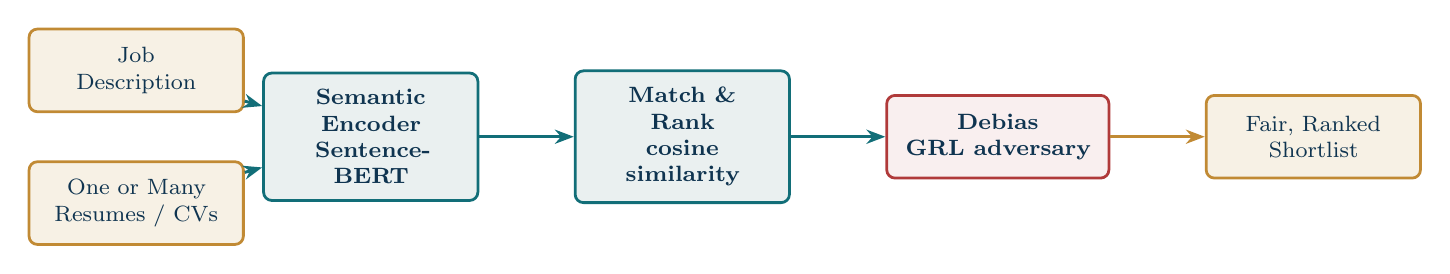
\begin{tikzpicture}[node distance=1.5cm and 1.2cm]
  \node[data,text width=2.3cm] (jd) {Job\\Description};
  \node[data,text width=2.3cm,below=0.6cm of jd] (cv) {One or Many\\Resumes / CVs};
  \node[stage,text width=2.3cm,right=1.6cm of $(jd)!0.5!(cv)$] (enc) {Semantic\\Encoder\\\footnotesize Sentence-BERT};
  \node[stage,text width=2.3cm,right=of enc] (match) {Match \&\\Rank\\\footnotesize cosine similarity};
  \node[stage,text width=2.4cm,right=of match,fill=TPred!8,draw=TPred] (deb) {Debias\\\footnotesize GRL adversary};
  \node[data,text width=2.3cm,right=of deb,fill=TPlightgold] (out) {Fair, Ranked\\Shortlist};
  \draw[fl] (jd) -- (enc);
  \draw[fl] (cv) -- (enc);
  \draw[fl] (enc) -- (match);
  \draw[fl] (match) -- (deb);
  \draw[flg] (deb) -- (out);
\end{tikzpicture}}
\caption{Module 1 at a glance: a job description and a candidate pool are ranked by semantic fit, then corrected for demographic influence before a final shortlist is produced.}
\label{fig:mod1-overview}
\end{figure}

\subsection{Datasets}
\label{sec:mod1-data}

Three purpose-built datasets underpin Module 1, summarized in Table~\ref{tab:mod1-data}. None of the three overlap in content; each was built for a distinct stage of the pipeline.

\begin{table}[H]
\centering
\caption{Module 1 datasets}
\label{tab:mod1-data}
\small
\begin{tabular}{p{2.9cm}p{1.6cm}p{1.6cm}p{8.5cm}}
\toprule
\hdrow \hdtxt{Dataset} & \hdtxt{Rows} & \hdtxt{Cols} & \hdtxt{Description} \\
\midrule
\code{resume.csv} & 1{,}125 & 2 & Core resume corpus across 49 job categories, used to train and evaluate the matcher. \\
\rowcolor{TPlight}
\code{job\_description.csv} & 147 & 2 & Job posting bank, exactly 3 postings per category spanning junior, mid, and senior seniority. \\
\code{BiasDataset.csv} & 1{,}960 & 8 & Demographically annotated resume corpus, 40 resumes per category, used exclusively for adversarial debiasing. \\
\bottomrule
\end{tabular}
\end{table}

\subsubsection{Resume Corpus (\code{resume.csv})}

The corpus originates from a public Kaggle resume dataset covering 14 classical software-engineering categories (Java Developer, Python Developer, DotNet Developer, Web Designing, Testing, Automation Testing, Data Science, Database, DevOps Engineer, Network Security Engineer, ETL Developer, SAP Developer, Hadoop, Blockchain). To reflect the modern technology job market, this was extended with 35 additional categories synthetically generated with Claude AI, spanning roles such as Product Manager, ML Engineer, MLOps Engineer, AI Engineer, Computer Vision Engineer, NLP Engineer, DevSecOps Engineer, Penetration Tester, UX Researcher, and Site Reliability Engineer, among others, bringing the total to 49 categories. The resume count per category is intentionally non-uniform, ranging from roughly 7 resumes for newer, synthetically generated categories up to roughly 80 for the original, well-represented categories such as Testing and DevOps Engineer, reflecting the underlying source distribution rather than an artificially balanced sample. Average resume length across the corpus is approximately 319 words.

\subsubsection{Job Description Bank (\code{job\_description.csv})}

All 147 job descriptions were authored by Claude AI to reflect realistic industry postings, with exactly three per category corresponding to junior, mid, and senior seniority levels, and an average length of approximately 38 words. Providing three job descriptions per category, rather than one, was a deliberate design choice: during training, a resume is paired with multiple job descriptions from its own category as positive examples, which prevents the matching model from memorizing a single template posting per category rather than learning genuine semantic alignment.

\subsubsection{Demographically Annotated Dataset (\code{BiasDataset.csv})}

This dataset was purpose-built for the debiasing stage and does not overlap with \code{resume.csv}. It was constructed in two phases: an original set of 20 categories $\times$ 40 resumes (800 rows), created with explicit demographic annotations and bias-reflective hiring outcomes to simulate a discriminatory HR process, followed by an extension to the remaining 29 categories (an additional 1{,}160 rows), generated with Claude AI while deliberately preserving the same demographic distribution proportions as the original 20 categories, so that the injected bias structure remains consistent across all 49 categories. Table~\ref{tab:mod1-demo} summarizes the demographic composition of the full dataset.

\begin{table}[H]
\centering
\caption{Demographic composition of \code{BiasDataset.csv} (1{,}960 rows total)}
\label{tab:mod1-demo}
\small
\begin{tabular}{p{2.6cm}p{4.4cm}p{1.6cm}p{1.6cm}}
\toprule
\hdrow \hdtxt{Attribute} & \hdtxt{Group} & \hdtxt{Count} & \hdtxt{\%} \\
\midrule
\multirow{2}{*}{Gender} & Male & 1{,}009 & 51.5 \\
 & Female & 951 & 48.5 \\
\rowcolor{TPlight}
\multirow{3}{*}{\cellcolor{TPlight}Skin colour} & Fair & 798 & 40.7 \\
\rowcolor{TPlight}
 & Medium & 672 & 34.3 \\
\rowcolor{TPlight}
 & Dark & 490 & 25.0 \\
\multirow{6}{*}{Ethnicity} & Bengali & 1{,}449 & 73.9 \\
 & Santal & 114 & 5.8 \\
 & Marma & 108 & 5.5 \\
 & Chakma & 104 & 5.3 \\
 & Garo & 95 & 4.8 \\
 & Manipuri & 90 & 4.6 \\
\rowcolor{TPlight}
\multirow{2}{*}{\cellcolor{TPlight}University tier} & Tier 1 (BUET, DU, BRAC, NSU, \ldots) & $\sim$1{,}101 & $\sim$56 \\
\rowcolor{TPlight}
 & Tier 2/3 (Daffodil, National Univ., \ldots) & $\sim$859 & $\sim$44 \\
\multirow{2}{*}{Hiring outcome} & Hired & 951 & 48.5 \\
 & Rejected & 1{,}009 & 51.5 \\
\bottomrule
\end{tabular}
\end{table}

The dataset carries two intentionally injected bias signals, described fully in Section~\ref{sec:mod1-biasinjection}: a binary \code{HiringDecision} label and a continuous \code{BiasedScore} field with mean 0.899 and range $[0.489, 1.000]$.

\subsection{Matching Model Architecture}
\label{sec:mod1-model}

The matching model is \code{all-MiniLM-L6-v2}, a distilled Sentence-BERT encoder, chosen after comparing three candidates:

\begin{itemize}[leftmargin=1.4cm]
  \item \code{all-mpnet-base-v2}: higher embedding quality (768 dimensions) but 110M parameters, making training and inference meaningfully slower for a 49-category matching task where that extra capacity was not judged necessary.
  \item \code{all-MiniLM-L6-v2}: 22.7M parameters, a 384-dimensional output embedding, and already strong baseline performance on semantic-similarity benchmarks. \textbf{Selected.}
  \item \code{paraphrase-multilingual-MiniLM-L12-v2}: multilingual support, relevant in principle to the Bangladeshi context, but adds unnecessary complexity since all corpus text is in English.
\end{itemize}

Sentence-BERT extends a pretrained BERT encoder with a Siamese or triplet-network training objective: two (or three) copies of the same encoder, sharing weights, independently embed two (or three) input texts, a pooling operation (mean pooling over token embeddings, in this configuration) reduces each variable-length token sequence to one fixed-size sentence vector, and a similarity-based loss is computed over the resulting vector pair. This architecture makes embedding computation for a single resume or job description a single forward pass, independent of what it will later be compared against, so a corpus of embeddings can be computed once and reused for many comparisons, which is essential for the ranking use case described in Section~\ref{sec:mod1-inference}.

Given two encoded texts, the resume embedding $\mathbf{e}_R \in \mathbb{R}^{384}$ and the job-description embedding $\mathbf{e}_J \in \mathbb{R}^{384}$, the match score is their cosine similarity:

\begin{formulabox}
\begin{equation}
\label{eq:cosine}
\mathrm{sim}(R,J) \;=\; \cos(\mathbf{e}_R, \mathbf{e}_J) \;=\; \frac{\mathbf{e}_R \cdot \mathbf{e}_J}{\lVert\mathbf{e}_R\rVert\,\lVert\mathbf{e}_J\rVert}
\end{equation}
\end{formulabox}

which, for the normalized embeddings produced by this model, lies in $[-1,1]$ and empirically clusters in $[0,1]$ for semantically related professional text. A validation-tuned decision threshold of $0.62$ separates matching from non-matching pairs; this threshold is derived empirically in Section~\ref{sec:mod1-results}.

\subsection{Training Pair Construction}
\label{sec:mod1-pairs}

Naively pairing every resume with a random wrong-category job description produces a training signal that is too easy: a Java Developer resume against a Game Developer posting is trivially dissimilar, and a model trained only on such pairs learns to reject obviously unrelated postings without ever learning the fine-grained distinctions that matter in practice. To force the model to learn genuinely discriminative representations, thirteen \emph{hard-negative groups} of semantically adjacent categories were defined, listed in Table~\ref{tab:mod1-hardneg}; a ``wrong category'' job description drawn from within the same group as a resume's true category is a hard negative, since it superficially resembles the resume's field without actually being the correct posting.

\begin{table}[H]
\centering
\caption{The thirteen hard-negative category groups used in training-pair construction}
\label{tab:mod1-hardneg}
\small
\begin{tabular}{p{2.9cm}p{10.7cm}}
\toprule
\hdrow \hdtxt{Group} & \hdtxt{Member categories} \\
\midrule
\code{core\_dev} & Java, Python, DotNet, Backend, Full Stack Developer \\
\rowcolor{TPlight}
\code{web\_frontend} & Web Designing, Frontend Developer, UI/UX Designer \\
\code{ai\_ml} & Data Science, ML Engineer, MLOps Engineer, AI Engineer, Applied AI Specialist \\
\rowcolor{TPlight}
\code{data\_platform} & Data Engineer, ETL Developer, Data Analyst, BI Analyst \\
\code{security} & AppSec, DevSecOps, Penetration Tester, Ethical Hacker, SOC Analyst, Network Security Engineer \\
\rowcolor{TPlight}
\code{cloud\_infra} & DevOps Engineer, Cloud Engineer, Platform Engineer, SRE, Cloud Architect \\
\code{arch} & Software Architect, Solutions Architect \\
\rowcolor{TPlight}
\code{mobile} & iOS Developer, Android Developer, Mobile Application Developer \\
\code{nlp\_cv} & NLP Engineer, Computer Vision Engineer \\
\rowcolor{TPlight}
\code{testing\_qa} & Testing, Automation Testing, QA Engineer \\
\code{management} & Product Manager, Technical Product Manager, Scrum Master \\
\rowcolor{TPlight}
\code{systems} & Embedded Systems Engineer, IoT Engineer \\
\code{product\_design} & UX Researcher, UI/UX Designer \\
\bottomrule
\end{tabular}
\end{table}

Each resume contributes eight pairs to the training set, summarized in Table~\ref{tab:mod1-pairconstruction}, yielding a positive-to-negative ratio of $1:1.66$, which deliberately over-represents negatives relative to positives, reflecting the reality that most candidates are not a fit for any given posting in real-world screening.

\begin{table}[H]
\centering
\caption{Training pair construction per resume, and the resulting corpus totals}
\label{tab:mod1-pairconstruction}
\small
\begin{tabular}{p{6.4cm}p{2.0cm}p{1.6cm}p{2.0cm}}
\toprule
\hdrow \hdtxt{Pair type} & \hdtxt{Per resume} & \hdtxt{Label} & \hdtxt{Total} \\
\midrule
Positive (resume $+$ same-category JD) & 3 & $y=1$ & 3{,}375 \\
\rowcolor{TPlight}
Hard negative (resume $+$ same-group, different-category JD) & 2 & $y=0$ & 2{,}220 \\
Random negative (resume $+$ random other-category JD) & 3 & $y=0$ & 3{,}375 \\
\midrule
\textbf{Total} & \textbf{8} & & \textbf{8{,}970} \\
\bottomrule
\end{tabular}
\end{table}

The train/validation/test split was performed at the \emph{resume level}, not the pair level, specifically to prevent data leakage: every pair generated from a given resume is guaranteed to land in the same split as that resume, so the model is never evaluated on a job-description pairing derived from a resume it has already seen during training. Table~\ref{tab:mod1-split} shows the resulting split, with an almost identical positive ratio preserved across all three partitions, confirming no stratification artefact was introduced.

\begin{table}[H]
\centering
\caption{Resume-level train/validation/test split}
\label{tab:mod1-split}
\small
\begin{tabular}{lrrr}
\toprule
\hdrow \hdtxt{Split} & \hdtxt{Resumes} & \hdtxt{Pairs} & \hdtxt{Positive ratio} \\
\midrule
Train & 900 (80\%) & 7{,}176 & 37.63\% \\
\rowcolor{TPlight}
Validation & 112 (10\%) & 893 & 37.63\% \\
Test & 113 (10\%) & 901 & 37.62\% \\
\bottomrule
\end{tabular}
\end{table}

\subsection{Training Configuration and Loss Function}
\label{sec:mod1-training}

The model was fine-tuned using \emph{MultipleNegativesRankingLoss}, an in-batch negative sampling loss closely related to the InfoNCE / NT-Xent objective used widely in contrastive representation learning. For a mini-batch of $N$ (anchor, positive) pairs $\{(a_i, p_i)\}_{i=1}^{N}$, every other positive $p_j$ ($j \ne i$) in the same batch is treated as an implicit negative for anchor $a_i$, without needing to be explicitly labelled as such. Writing $s_{ij} = \mathrm{sim}(a_i, p_j)$ for the cosine similarity between anchor $i$ and candidate $j$, and $\tau$ for a fixed temperature (equivalently, a similarity scale factor), the loss for the batch is:

\begin{formulabox}
\begin{equation}
\label{eq:mnrl}
\mathcal{L}_{\mathrm{MNRL}} \;=\; -\frac{1}{N}\sum_{i=1}^{N} \log \frac{\exp\!\big(s_{ii}/\tau\big)}{\sum_{j=1}^{N}\exp\!\big(s_{ij}/\tau\big)}
\end{equation}
\end{formulabox}

which is a softmax cross-entropy loss over each row of the in-batch similarity matrix, pushing the true pairing $s_{ii}$ to be the largest value in its row relative to every other candidate in the batch. With a batch size of 32, this construction generates $32 \times 31 = 992$ pairwise ranking constraints from a single batch, which is markedly more sample-efficient than a simple binary classification loss evaluated pair by pair. Table~\ref{tab:mod1-hyperparams} lists the full training configuration.

\begin{table}[H]
\centering
\caption{Module 1 matching-model training configuration}
\label{tab:mod1-hyperparams}
\small
\begin{tabular}{p{3.2cm}p{3.3cm}p{6.9cm}}
\toprule
\hdrow \hdtxt{Hyperparameter} & \hdtxt{Value} & \hdtxt{Rationale} \\
\midrule
Loss function & Multiple\-Negatives\-Ranking\-Loss & Ranking-based, in-batch negative sampling (Equation~\ref{eq:mnrl}) \\
\rowcolor{TPlight}
Epochs & 10 & Validation Spearman correlation plateaus by epoch 7--8 \\
Batch size & 32 & Balances GPU utilization against in-batch negative diversity \\
\rowcolor{TPlight}
Warm-up steps & 85 ($\approx$ 1 epoch) & One full epoch of linear learning-rate warm-up to protect pretrained weights from early destructive updates \\
Training triplets & 2{,}700 & (anchor, positive, hard-negative) triplets drawn from Section~\ref{sec:mod1-pairs} \\
\rowcolor{TPlight}
Evaluator & Embedding\-Similarity\-Evaluator & Run each epoch on the validation split; best checkpoint retained by Spearman correlation \\
\bottomrule
\end{tabular}
\end{table}

Figure~\ref{fig:mod1-training} traces this whole construction process end to end, from the two raw source files through to the deployed matcher used at inference time.

\begin{figure}[H]
\centering
\resizebox{\linewidth}{!}{%
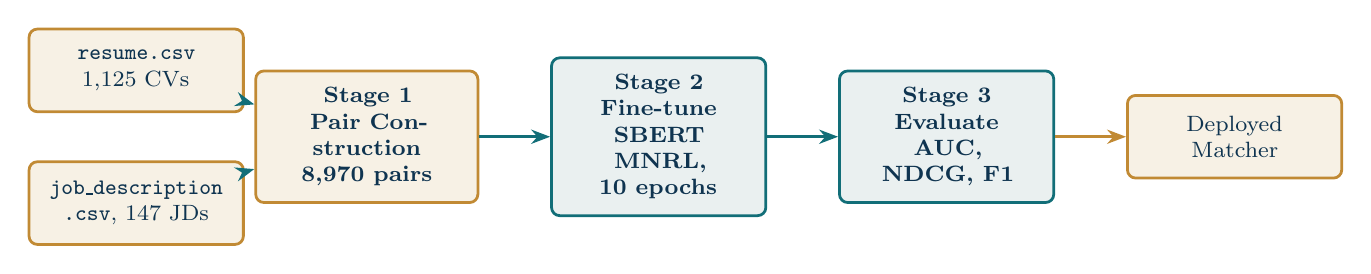
\begin{tikzpicture}[node distance=1.3cm and 0.9cm]
  \node[data,text width=2.3cm] (r) {\code{resume.csv}\\1{,}125 CVs};
  \node[data,text width=2.3cm,below=0.6cm of r] (j) {\code{job\_description}\\\code{.csv}, 147 JDs};
  \node[stage,text width=2.4cm,right=1.5cm of $(r)!0.5!(j)$,fill=TPlightgold,draw=TPgold] (pair) {Stage 1\\Pair Construction\\\footnotesize 8{,}970 pairs};
  \node[stage,text width=2.3cm,right=of pair] (train) {Stage 2\\Fine-tune SBERT\\\footnotesize MNRL, 10 epochs};
  \node[stage,text width=2.3cm,right=of train] (eval) {Stage 3\\Evaluate\\\footnotesize AUC, NDCG, F1};
  \node[data,text width=2.3cm,right=of eval,fill=TPlightgold] (dep) {Deployed\\Matcher};
  \draw[fl] (r) -- (pair);
  \draw[fl] (j) -- (pair);
  \draw[fl] (pair) -- (train);
  \draw[fl] (train) -- (eval);
  \draw[flg] (eval) -- (dep);
\end{tikzpicture}}
\caption{How the matching model itself was built: the two raw source files are turned into training pairs, used to fine-tune the encoder, evaluated on the held-out split, and shipped as the deployed matcher.}
\label{fig:mod1-training}
\end{figure}

\subsubsection{Training Dynamics}

Table~\ref{tab:mod1-curves} records the validation Spearman and Pearson correlation between predicted similarity and ground-truth label at every epoch. The largest single improvement occurs between epochs 1 and 2 ($+0.028$ Spearman), corresponding to the model's rapid adaptation from general-purpose language understanding to the specific vocabulary and phrasing of resumes and job descriptions; the curve then improves steadily but with diminishing returns through epoch 10, with no epoch-over-epoch decrease at any point, indicating the warm-up schedule and the model's inherent regularization were sufficient to avoid overfitting within this training budget.

\begin{table}[H]
\centering
\caption{Validation metric progression across training}
\label{tab:mod1-curves}
\small
\begin{tabular}{cccc}
\toprule
\hdrow \hdtxt{Epoch} & \hdtxt{Spearman} & \hdtxt{Pearson} & \\
\midrule
1 & 0.8044 & 0.8441 & \\
\rowcolor{TPlight}
2 & 0.8320 & 0.8959 & \\
3 & 0.8340 & 0.9040 & \\
\rowcolor{TPlight}
4 & 0.8363 & 0.9167 & \\
5 & 0.8367 & 0.9199 & \\
\rowcolor{TPlight}
6 & 0.8374 & 0.9216 & \\
7 & 0.8378 & 0.9279 & \\
\rowcolor{TPlight}
8 & 0.8380 & 0.9268 & \\
9 & 0.8383 & 0.9266 & \\
\rowcolor{TPlight}
\textbf{10 (best)} & \textbf{0.8383} & \textbf{0.9274} & \\
\bottomrule
\end{tabular}
\end{table}

\subsection{Evaluation Metrics and Test-Set Results}
\label{sec:mod1-results}

Four metrics were used to characterize the trained matcher, each measuring a distinct property of its output.

\textbf{AUC-ROC} measures how well the model separates matching from non-matching pairs across every possible decision threshold simultaneously; a score of 1.0 indicates that every positive pair scores higher than every negative pair, regardless of threshold, and 0.5 indicates performance no better than random guessing. \textbf{NDCG@10} evaluates ranking quality: for a given resume, it asks whether the truly matching job descriptions appear near the top of a ranked list of candidates, with a correct match at rank 1 weighted more heavily than one at rank 10; a score of 1.0 means every relevant job description outranks every irrelevant one within the top 10 results, for every resume evaluated. \textbf{F1} is the harmonic mean of precision (of everything the system flagged as a match, how much actually was) and recall (of everything that truly matched, how much the system found). The \textbf{cosine similarity gap} is the mean similarity of positive pairs minus the mean similarity of negative pairs, a direct measure of how cleanly the embedding space separates the two classes.

\begin{table}[H]
\centering
\caption{Module 1 matcher: full test-set results (901 pairs: 339 positive, 562 negative)}
\label{tab:mod1-results}
\small
\begin{tabular}{lr}
\toprule
\hdrow \hdtxt{Metric} & \hdtxt{Value} \\
\midrule
AUC-ROC & \textbf{0.9998} \\
\rowcolor{TPlight}
NDCG@10 & \textbf{1.0000} \\
F1 (optimal threshold $=0.62$) & \textbf{0.9926} \\
\rowcolor{TPlight}
Accuracy (optimal threshold) & \textbf{0.9945} \\
F1 (threshold $=0.50$) & 0.9603 \\
\rowcolor{TPlight}
Accuracy (threshold $=0.50$) & 0.9689 \\
Mean positive-pair similarity & 0.8508 \\
\rowcolor{TPlight}
Mean negative-pair similarity & 0.2294 \\
\textbf{Cosine similarity gap} & \textbf{0.6214} \\
\rowcolor{TPlight}
Categories at AUC $=1.0$, NDCG@10 $=1.0$ & 48 of 48 evaluated \\
\bottomrule
\end{tabular}
\end{table}

An AUC of 0.9998 means that, drawing one matching pair and one non-matching pair at random, the matching pair scores higher 99.98\% of the time, effectively a solved discrimination task on this evaluation set. A perfect NDCG@10 of 1.000 means that across every resume tested, the model never once ranked an irrelevant job description above a relevant one within the top ten results, which is the property that matters most for a real screening system, since it directly controls whether a genuinely suitable candidate is ever pushed out of view. The similarity gap of 0.621, an average of 0.851 for true matches against 0.229 for non-matches, indicates a wide, clean margin between the two classes; the chosen decision threshold of 0.62 sits close to the midpoint of this gap, consistent with a genuinely bimodal, well-separated score distribution rather than one requiring a finely tuned cutoff.

Category-level performance varies with vocabulary specificity, as shown in Table~\ref{tab:mod1-percategory}. Categories built around proprietary or highly specific technical vocabulary (SAP, Hadoop) separate most cleanly, while categories whose technology stacks genuinely overlap with neighbouring roles (Mobile Development, Network Security, Site Reliability Engineering) show a smaller similarity gap, even though every one of the 48 evaluated categories still achieves a perfect AUC and NDCG@10, meaning the \emph{ranking} remains flawless even where the absolute score margin is narrower.

\begin{table}[H]
\centering
\caption{Selected per-category results illustrating the range of task difficulty}
\label{tab:mod1-percategory}
\small
\begin{tabular}{p{3.4cm}rrrp{4.6cm}}
\toprule
\hdrow \hdtxt{Category} & \hdtxt{Pos.\ sim.} & \hdtxt{Neg.\ sim.} & \hdtxt{Gap} & \hdtxt{Note} \\
\midrule
SAP Developer & 0.918 & 0.105 & \textbf{0.814} & Highest gap; SAP vocabulary is highly specialized \\
\rowcolor{TPlight}
Hadoop & 0.922 & 0.181 & 0.741 & Distinctive terms (MapReduce, Hive, HDFS) \\
BI Analyst & 0.904 & 0.164 & 0.740 & Power BI / data-warehouse vocabulary separates cleanly \\
\rowcolor{TPlight}
Mobile App Developer & 0.827 & 0.363 & 0.464 & Lowest gap; overlaps with Frontend Development \\
Network Security Eng. & 0.677 & 0.208 & 0.469 & Niche vocabulary underrepresented in pretraining \\
\rowcolor{TPlight}
Site Reliability Eng. & 0.703 & 0.138 & 0.565 & Overlaps heavily with DevOps vocabulary \\
\bottomrule
\end{tabular}
\end{table}

\subsection{Inference and the Fair-Screening Report}
\label{sec:mod1-inference}

At inference time, both texts are encoded independently, the cosine similarity of Equation~\ref{eq:cosine} is computed, and the full candidate pool for a given posting is ranked. In the deployed system, invoking ``Fair-Screen Candidates'' produces a ten-part report, summarized in Table~\ref{tab:mod1-report}, that walks an HR administrator from the raw parsed profile of every candidate through to a final, debiased shortlist decision.

\begin{table}[H]
\centering
\caption{The ten stages of the deployed Fair-Screening report}
\label{tab:mod1-report}
\small
\begin{tabular}{cp{3.2cm}p{9.4cm}}
\toprule
\hdrow \hdtxt{\#} & \hdtxt{Stage} & \hdtxt{Content} \\
\midrule
1 & Profiles & The four factors parsed off each CV: university, gender, ethnicity, skin colour \\
\rowcolor{TPlight}
2 & First reading & Each candidate's raw similarity score and rank, before any correction \\
3 & Attribution & Points added or subtracted by background alone, per candidate \\
\rowcolor{TPlight}
4 & Residual & The same four factors, re-measured on the debiased score \\
5 & Per-person detail & The same figures narrated one candidate at a time \\
\rowcolor{TPlight}
6 & Fair reading & Every candidate re-ranked using only the debiased score \\
7 & Comparison & Original and corrected scores shown side by side \\
\rowcolor{TPlight}
8 & Fairness impact & Percentage of the batch's score spread attributable to background, and how much the correction closed \\
9 & Movement & Who moved up or down the most, and why \\
\rowcolor{TPlight}
10 & Decision & Shortlist / Reject / Undo, with the debiased model's own recommended score bands \\
\bottomrule
\end{tabular}
\end{table}

The recommended score bands surfaced at stage 10, namely 95\% and above as highly probable, 62\% and above as shortlisted, 55\% and above as a weak match, and below 55\% as rejected, are a recommendation rather than an enforced rule; the shortlist and reject controls function regardless of what the model suggests, so an administrator retains the final decision in every case.

\subsubsection{Live Inference Demonstration}

Two worked examples illustrate the matcher's behaviour concretely, rather than only through aggregate test-set statistics. In the first, a single resume for Tanvir Hasan, a senior Python developer, was scored against two different job descriptions: a Python backend posting returned a similarity of $0.8246$ (a match), while an iOS Developer posting returned $0.2275$ (not a match), a gap of $0.597$ that correctly separates the right role from an unrelated one for the same candidate.

The second example ranks four candidates of visibly different backgrounds against one Data Scientist posting, shown in Table~\ref{tab:mod1-demo-rank}.

\begin{table}[H]
\centering
\caption{Ranking four candidates against a Data Scientist job description}
\label{tab:mod1-demo-rank}
\small
\begin{tabular}{cccp{3.6cm}l}
\toprule
\hdrow \hdtxt{Rank} & \hdtxt{Score} & \hdtxt{Candidate} & \hdtxt{Background} & \hdtxt{Verdict} \\
\midrule
1 & \textbf{0.9268} & Fatema Akter & Data Science, BUET & Match \\
\rowcolor{TPlight}
2 & 0.6695 & Nasreen Sultana & Data Analyst, NSU & Match \\
3 & 0.5469 & Arif Rahman & ML Engineer, DU & Weak match \\
\rowcolor{TPlight}
4 & 0.0700 & Rahim Uddin & Java Developer, CUET & No match \\
\bottomrule
\end{tabular}
\end{table}

The ranking surfaces the strongest fit at the top, correctly identifies an adjacent but not identical role (an ML Engineer applying for a Data Scientist opening) as only a weak match rather than either a strong match or an outright rejection, and cleanly rejects a candidate from an unrelated field. This is the practical behaviour the aggregate metrics of Table~\ref{tab:mod1-results} are summarizing: the model does not just separate matches from non-matches at the extremes, it orders the middle ground sensibly too.

\subsection{Skill Extraction Service}
\label{sec:mod1-skillex}

A companion service, independent from the ranking model, performs skill extraction from both resumes and job descriptions using GLiNER, a zero-shot named-entity recognition model that identifies text spans matching a supplied list of free-text category labels without requiring retraining for new skill vocabularies. Extracted skills are used to populate the ``Skills this job needs'' and per-candidate matched/missing/extra skill breakdown surfaced in the application, described further in Section~\ref{sec:frontend}, and are computed independently of the ranking score itself. This same GLiNER-based extraction approach is reused, with a differently configured label set, in Module 2, and is described in full architectural and formula detail in Section~\ref{sec:mod2-extraction} rather than repeated here.

A separate, rule-based component, \code{biasExtractor.js}, parses the raw CV text for the four demographic factors used throughout this section: name (the first non-blank line, up to a dash or pipe), university tier (matched against an alias table; BUET, DU, and BRAC are Tier 1, CUET/RUET/KUET/SUST/JU/NSU are Tier 2, and any other named university, institute, or college is Tier 3), gender (matched against a Bangladeshi-name dictionary, with an optional large-language-model fallback), and ethnicity (read in priority order from an explicit ``(Native)'' language tag, an explicit community-membership sentence, a surname match, and finally a Bengali default, recognizing six classes: Bengali, Chakma, Garo, Manipuri, Marma, and Santal). Skin colour is documented explicitly, both here and to any user of the system, as a simulation-only field: it requires an explicit ``Skin Colour: Fair/Medium/Dark'' line that no real resume would ever contain, present solely so the debiased model (which was trained expecting that feature) has a defined value to work against; if absent, it contributes nothing to either score. This transparency about which parts of the pipeline are genuine document understanding and which are a deliberate research simulation is treated as a requirement of this report, not an afterthought.

\subsection{Adversarial Debiasing}
\label{sec:mod1-debias}

This subsection presents the adversarial debiasing mechanism designed to decouple demographic signals from candidate competence, detailing bias injection, adversarial architecture, and fairness evaluation.

\subsubsection{Motivation}

A matching model trained purely on textual content, as described in Sections~\ref{sec:mod1-model}--\ref{sec:mod1-results}, is not automatically fair once deployed inside a real hiring workflow, nor when trained (as many real-world systems are) on historical decisions that themselves encode human bias. To both demonstrate and directly address this, three things were done: an intentionally biased dataset was constructed (Section~\ref{sec:mod1-biasinjection}), an adversarial system was trained to detect and actively remove demographic signal from the shared embedding space (Section~\ref{sec:mod1-grl}), and the resulting bias, before and after, was measured with standardized fairness metrics (Section~\ref{sec:mod1-fairnessresults}).

\subsubsection{Bias Injection Design}
\label{sec:mod1-biasinjection}

Two forms of bias were deliberately injected into \code{BiasDataset.csv} to create a controlled baseline against which the debiasing procedure could be measured.

\textbf{HiringDecision}, a binary label, was generated from a probabilistic formula that discriminates along four axes simultaneously:

\begin{formulabox}
\begin{align}
\label{eq:hiring}
p_{\text{base}} &= \begin{cases} 0.75 & \text{university Tier 1} \\ 0.50 & \text{Tier 2} \\ 0.25 & \text{Tier 3} \end{cases} \nonumber \\
p &= \mathrm{clip}\big(p_{\text{base}} + \delta_{\text{gender}} + \delta_{\text{skin}} + \delta_{\text{ethnicity}},\; 0.05,\; 0.95\big)
\end{align}
\end{formulabox}

where $\delta_{\text{gender}} = +0.15$ for male and $-0.15$ for female, $\delta_{\text{skin}} = +0.10$ for fair and $-0.10$ for dark, and $\delta_{\text{ethnicity}} = +0.10$ for Bengali and $-0.15$ for a minority ethnicity, and \code{HiringDecision} is then a Bernoulli draw with success probability $p$. A Tier-1, male, fair-skinned, Bengali candidate reaches a hiring probability of $0.75+0.15+0.10+0.10=1.10$, clamped to the ceiling of 0.95; a Tier-3, female, dark-skinned, minority-ethnicity candidate reaches $0.25-0.15-0.10-0.15=-0.15$, clamped to the floor of 0.05, a nineteen-to-one odds ratio between two candidates who may hold identical qualifications.

\textbf{BiasedScore}, a continuous field simulating what a biased model's own similarity output might look like, follows the same directional pattern at smaller magnitude:

\begin{formulabox}
\begin{equation}
\label{eq:biasedscore}
\mathrm{BiasedScore} = \mathrm{clip}\big(\mathcal{N}(0.93,\,0.025^2) + \delta'_{\text{uni}} + \delta'_{\text{gender}} + \delta'_{\text{skin}} + \delta'_{\text{ethnicity}},\; 0,\; 1\big)
\end{equation}
\end{formulabox}

with individual adjustments in the range $\pm0.05$ to $\pm0.15$, representing a subtler form of bias that might arise in a trained model without anyone explicitly programming it in.

\subsubsection{Adversarial Architecture: Gradient Reversal}
\label{sec:mod1-grl}

The debiasing procedure uses adversarial training with a Gradient Reversal Layer (GRL), a technique originally developed for unsupervised domain adaptation (Ganin and Lempitsky, 2015) and repurposed here for fairness. The GRL is defined by an identity mapping on the forward pass and a sign-reversed, scaled gradient on the backward pass:

\begin{formulabox}
\begin{equation}
\label{eq:grl}
R_\lambda(\mathbf{x}) = \mathbf{x}, \qquad \frac{\partial R_\lambda}{\partial \mathbf{x}} = -\lambda \mathbf{I}
\end{equation}
\end{formulabox}

where $\lambda \geq 0$ is a scheduled scalar controlling adversarial strength. Figure~\ref{fig:mod1-grl} shows the resulting architecture. The shared encoder (the same \code{all-MiniLM-L6-v2} architecture from Section~\ref{sec:mod1-model}) produces one embedding per resume; this embedding feeds two paths simultaneously. On the normal path, a CosineEmbeddingLoss between resume and job-description embeddings preserves the matching capability learned in Section~\ref{sec:mod1-training}. On the adversarial path, the embedding passes through the GRL and into four independent adversary networks, one per demographic attribute (gender, university tier, skin colour, ethnicity), each with the architecture \code{Linear(384,256)} $\to$ \code{ReLU} $\to$ \code{Dropout(0.3)} $\to$ \code{Linear(256,}$n_c$\code{)}, where $n_c$ is 2, 3, 3, and 6 respectively.

\begin{figure}[H]
\centering
\resizebox{0.9\linewidth}{!}{%
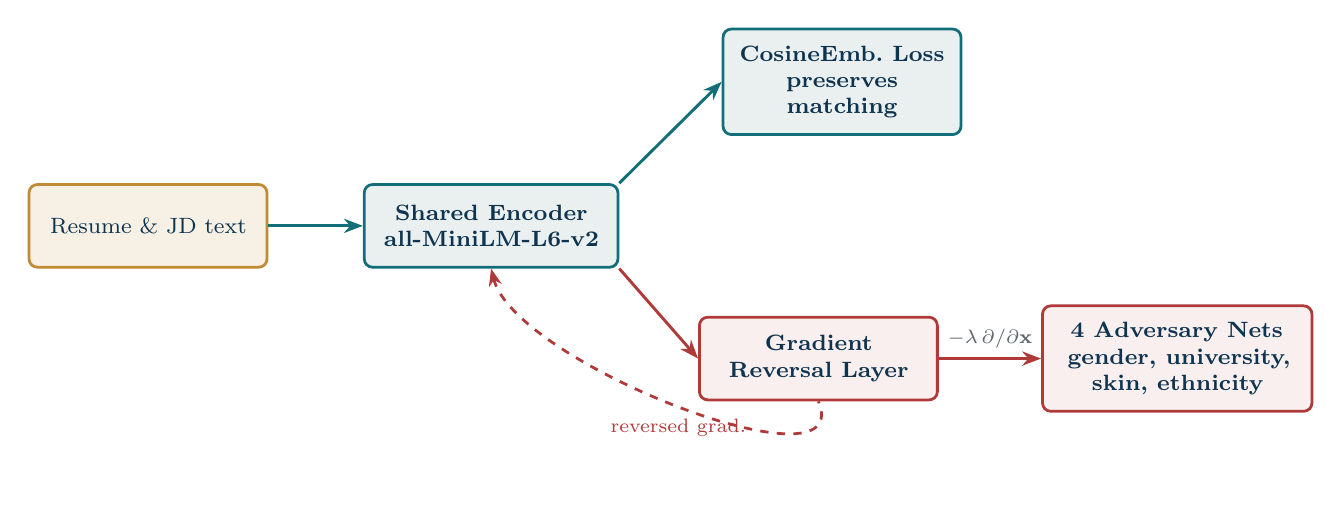
\begin{tikzpicture}[node distance=1.0cm]
  \node[data,text width=2.6cm] (in) {Resume \& JD text};
  \node[stage,text width=2.8cm,right=1.2cm of in] (enc) {Shared Encoder\\\footnotesize all-MiniLM-L6-v2};
  \node[stage,text width=2.6cm,above right=0.6cm and 1.3cm of enc,fill=TPlight] (cos) {CosineEmb.\ Loss\\\footnotesize preserves matching};
  \node[stage,text width=2.6cm,below right=0.6cm and 1.0cm of enc,fill=TPred!8,draw=TPred] (grl) {Gradient\\Reversal Layer};
  \node[stage,text width=3.0cm,right=1.3cm of grl,fill=TPred!8,draw=TPred] (adv) {4 Adversary Nets\\\footnotesize gender, university,\\skin, ethnicity};
  \draw[fl] (in) -- (enc);
  \draw[fl] (enc.north east) -- (cos.west);
  \draw[flr] (enc.south east) -- (grl.west);
  \draw[flr] (grl) -- node[above,note]{$-\lambda\,\partial/\partial\mathbf{x}$} (adv);
  \draw[{Stealth[length=2.2mm]}-,line width=1pt,draw=TPred,dashed]
        (enc.south) .. controls +(0.3,-1.2) and +(0.5,-1.2) .. (grl.south)
        node[midway,below=1pt,font=\scriptsize,text=TPred]{reversed grad.};
\end{tikzpicture}}
\caption{The adversarial debiasing architecture. The encoder is shared with the matching task; the Gradient Reversal Layer flips the sign of adversary gradients flowing back into the encoder, teaching it to hide demographic signal rather than expose it.}
\label{fig:mod1-grl}
\end{figure}

In plain terms, the system runs two competing objectives at once. The adversary networks learn, via ordinary gradient descent, to predict demographic attributes from the shared embedding. The encoder receives the adversaries' gradients with their sign flipped by the GRL, so instead of learning to make demographic signal \emph{easier} for the adversaries to detect (which is what would happen without reversal), it learns to make that signal \emph{harder} to detect, while the unmodified CosineEmbeddingLoss gradient continues to push it toward preserving genuine matching quality. This is formally a minimax game between the encoder and the adversaries, and the encoder is considered to have succeeded once the adversaries can no longer predict demographics better than random chance from its output.

\subsubsection{Training Procedure}

Training proceeds in two phases. \textbf{Phase A} (3 epochs) freezes the encoder entirely and trains only the four adversary networks on fixed, pre-computed embeddings. This step exists because reversing a gradient from an adversary that has not yet learned anything meaningful is a no-op; Phase A first gives the adversaries a genuine signal to detect before Phase B begins reversing it. By the end of Phase A, adversary training accuracies reached Gender $=0.584$, University $=0.451$, Skin colour $=0.402$, Ethnicity $=0.586$, each above the corresponding random-guess baseline, confirming the adversaries had learned real, if imperfect, demographic signal.

\textbf{Phase B} (12 epochs) unfreezes the encoder and trains both paths jointly. The adversarial strength $\lambda$ is scheduled to ramp from $1.18$ at epoch 4 to a ceiling of $1.50$ by epoch 9, so that adversarial pressure is applied gradually rather than destructively from the first step. The total loss combines the similarity-preservation term with the four (weighted) adversary cross-entropy losses:

\begin{formulabox}
\begin{equation}
\label{eq:total-loss}
\mathcal{L}_{\text{total}} \;=\; \mathcal{L}_{\text{sim}} \;+\; \mathcal{L}^{\text{gender}}_{\text{CE}} \;+\; \mathcal{L}^{\text{university}}_{\text{CE}} \;+\; \mathcal{L}^{\text{skin}}_{\text{CE}} \;+\; \mathcal{L}^{\text{ethnicity}}_{\text{CE}}
\end{equation}
\end{formulabox}

Table~\ref{tab:mod1-trainlog} records loss values sampled through Phase B; the similarity loss remains near zero throughout, confirming matching quality is preserved, while the adversary loss stays consistently high, confirming the adversaries remain genuinely confused rather than converging to a trivial solution.

\begin{table}[H]
\centering
\caption{Phase B training log (sampled epochs)}
\label{tab:mod1-trainlog}
\small
\begin{tabular}{ccccc}
\toprule
\hdrow \hdtxt{Epoch} & \hdtxt{$\lambda$} & \hdtxt{Sim.\ loss} & \hdtxt{Adv.\ loss} & \hdtxt{Total loss} \\
\midrule
4 & 1.1850 & 0.0580 & 4.6046 & 4.6626 \\
\rowcolor{TPlight}
7 & 1.4593 & 0.0404 & 4.6050 & 4.6454 \\
10 & 1.4952 & 0.0373 & 4.6140 & 4.6513 \\
\rowcolor{TPlight}
13 & 1.4994 & 0.0317 & 4.6127 & 4.6444 \\
15 & 1.4999 & 0.0268 & 4.6130 & 4.6398 \\
\bottomrule
\end{tabular}
\end{table}

\subsubsection{The Ethnicity Class-Imbalance Fix}

A specific implementation issue was identified and corrected during this phase. With standard, unweighted cross-entropy, the ethnicity adversary discovered a shortcut: predicting ``Bengali'' for every input achieves 73.9\% accuracy on its own, since Bengali constitutes 73.9\% of the dataset, without the adversary ever learning to distinguish the five minority classes. Since the GRL can only reverse a signal the adversary has actually learned, this left the encoder with no real pressure to hide minority-ethnicity signal specifically. The fix applied inverse-frequency class weights,

\begin{formulabox}
\begin{equation}
\label{eq:classweight}
w_c \;=\; \frac{n_{\text{total}}}{n_{\text{classes}} \times n_c}
\end{equation}
\end{formulabox}

giving the majority Bengali class a weight of $0.224$ and minority classes weights between $3.1$ and $3.6$, forcing the adversary to genuinely attempt to distinguish Chakma, Marma, Manipuri, Garo, and Santal resumes rather than defaulting to the majority label.

\subsection{Fairness Metrics}
\label{sec:mod1-fairnessdef}

Two standard fairness metrics, both defined over group-wise acceptance rates, are used to quantify bias before and after debiasing.

\textbf{Demographic Parity Difference (DPD)} is the gap between the most- and least-favoured group's acceptance rate:

\begin{formulabox}
\begin{equation}
\label{eq:dpd}
\mathrm{DPD} = \max_g \big(\Pr[\hat{y}=1 \mid G=g]\big) - \min_g \big(\Pr[\hat{y}=1 \mid G=g]\big)
\end{equation}
\end{formulabox}

A DPD of 0 is perfect parity; larger values indicate a larger worst-case gap between the most- and least-favoured demographic group. \textbf{Disparate Impact Ratio (DIR)} is the ratio of the worst- to best-treated group's acceptance rate:

\begin{formulabox}
\begin{equation}
\label{eq:dir}
\mathrm{DIR} = \frac{\min_g \big(\Pr[\hat{y}=1 \mid G=g]\big)}{\max_g \big(\Pr[\hat{y}=1 \mid G=g]\big)}
\end{equation}
\end{formulabox}

A DIR of 1.0 indicates perfectly equal treatment; the widely used United States EEOC ``four-fifths rule'' treats a system with DIR below 0.80 as showing evidence of adverse impact.

\subsection{Debiasing Results}
\label{sec:mod1-fairnessresults}

Table~\ref{tab:mod1-fairness} reports DPD and DIR before and after debiasing, for all four protected attributes.

\begin{table}[H]
\centering
\caption{Fairness metrics before and after adversarial debiasing}
\label{tab:mod1-fairness}
\small
\begin{tabular}{C{2.3cm}C{1.5cm}C{1.5cm}C{1.5cm}C{1.5cm}C{1.5cm}C{2.3cm}}
\toprule
\hdrow \hdtxt{Attribute} & \hdtxt{DPD before} & \hdtxt{DPD after} & \hdtxt{Reduction} & \hdtxt{DIR before} & \hdtxt{DIR after} & \hdtxt{4/5 rule} \\
\midrule
Gender & 0.2971 & \textbf{0.0359} & \textbf{$-$88\%} & 0.528 & \textbf{0.929} & \gd{Passes} \\
\rowcolor{TPlight}
University tier & 0.4752 & \textbf{0.0114} & \textbf{$-$98\%} & 0.398 & \textbf{0.977} & \gd{Passes} \\
Skin colour & 0.1646 & \textbf{0.0343} & \textbf{$-$79\%} & 0.704 & \textbf{0.931} & \gd{Passes} \\
\rowcolor{TPlightgold}
Ethnicity & 0.3307 & 0.1592 & $-$52\% & 0.399 & 0.710 & Below threshold \\
\bottomrule
\end{tabular}
\end{table}

Three of the four protected attributes clear the 0.80 legal threshold after correction, with demographic parity gaps reduced by 79--98\%. Table~\ref{tab:mod1-leakage} reports a complementary check: adversary leakage, the accuracy with which a freshly trained classifier can recover demographic attributes purely from the model's embedding, before and after debiasing.

\begin{table}[H]
\centering
\caption{Adversary leakage (classifier accuracy on demographics, from embeddings alone)}
\label{tab:mod1-leakage}
\small
\begin{tabular}{lccccc}
\toprule
\hdrow \hdtxt{Attribute} & \hdtxt{Before} & \hdtxt{After (sklearn probe)} & \hdtxt{After (adversary net)} & \hdtxt{Random} \\
\midrule
Gender & 0.822 & 0.583 & 0.531 & 0.500 \\
\rowcolor{TPlight}
University tier & 0.595 & 0.482 & 0.431 & 0.333 \\
Skin colour & 0.468 & 0.446 & 0.407 & 0.333 \\
\rowcolor{TPlight}
Ethnicity & 0.739 & 0.739 & \textbf{0.432} & 0.167 \\
\bottomrule
\end{tabular}
\end{table}

Gender leakage falls from 82.2\% to close to the 50\% random baseline. The debiased similarity-score distribution also compresses sharply: standard deviation across five demographically diverse but skill-identical demonstration candidates drops from 0.039 to 0.005, and the score spread between the highest- and lowest-scoring demo candidate collapses from 0.4500 to 0.0017, a 99.6\% reduction, with the previously lowest-scoring candidate gaining 0.4456 points and the previously highest-scoring candidate losing only 0.005 points, meaning the correction lifts the disadvantaged rather than penalizing the advantaged.

\subsection{Candidate Ranking Demonstration and Bias Attribution}
\label{sec:mod1-ranking-demo}

The aggregate figures above are best understood alongside a concrete case. Five demonstration candidates, each holding an identical skill profile (five years of Python, three years of AWS, three years of PostgreSQL, and so on) but differing only in demographic background, were ranked against a Data Analyst posting, first using the \code{BiasedScore} formula of Equation~\ref{eq:biasedscore} to stand in for a demographically influenced score, and then using the debiased model. Table~\ref{tab:mod1-candidate-demo} shows both readings side by side.

\begin{table}[H]
\centering
\caption{Five candidates with identical skills, ranked before and after debiasing}
\label{tab:mod1-candidate-demo}
\small
\begin{tabular}{p{3.4cm}p{5.4cm}cc}
\toprule
\hdrow \hdtxt{Candidate} & \hdtxt{Background} & \hdtxt{Score before} & \hdtxt{Score after} \\
\midrule
Arif Rahman & BUET, male, fair skin, Bengali & 1.0000 & 0.9949 \\
\rowcolor{TPlight}
Nasreen Akter & DU, female, medium skin, Bengali & 1.0000 & 0.9960 \\
Sajib Tripura & NSU, male, fair skin, Manipuri & 0.9400 & 0.9943 \\
\rowcolor{TPlight}
Rahim Uddin & Daffodil, male, dark skin, Bengali & 0.8300 & 0.9955 \\
Farida Chakma & National University, female, dark skin, Chakma & \textbf{0.5500} & \textbf{0.9956} \\
\bottomrule
\end{tabular}
\end{table}

Before correction, Farida Chakma, the candidate with the least-favoured background under every axis the injected bias formula rewards, scores 0.45 points below Arif Rahman despite an identical skill set. After correction, all five candidates cluster between 0.994 and 0.996, a score spread of 0.0017 against 0.4500 beforehand, a 99.6\% reduction. Farida Chakma's own score rises by 0.4456 points; Arif Rahman's falls by only 0.0051 points, which is the intended asymmetry: debiasing is meant to lift whoever was penalized for their background, not to punish whoever happened to benefit from it.

Two further checks isolate exactly which signal the correction removed. The first, summarized in Table~\ref{tab:mod1-swap}, swaps a single demographic attribute in Arif Rahman's resume text at a time (his university, for instance, from BUET to National University) and measures how much the model's score moves in response, both before and after debiasing.

\begin{table}[H]
\centering
\caption{Score change from swapping one demographic attribute in a resume's text}
\label{tab:mod1-swap}
\small
\begin{tabular}{lcccc}
\toprule
\hdrow \hdtxt{Attribute swapped} & \hdtxt{Bias before} & \hdtxt{Bias after} & \hdtxt{Removed} \\
\midrule
University & 0.0068 & 0.0001 & \textbf{98\%} \\
\rowcolor{TPlight}
Ethnicity & 0.0044 & 0.0002 & \textbf{94\%} \\
Gender & 0.0003 & 0.0004 & --- \\
\rowcolor{TPlight}
Skin colour & 0.0000 & 0.0000 & --- \\
\bottomrule
\end{tabular}
\end{table}

University and ethnicity were the two attributes the undebiased model had genuinely learned to read out of resume text, and both are almost entirely gone after correction. Gender and skin colour were never strongly encoded in the text in the first place, which is unsurprising: a text-based swap such as changing a pronoun captures gender only weakly compared to a name or a university name, so there was little text-encoded signal there to remove.

The second check asks a more individual question: for Farida Chakma specifically, can the trained adversary networks still guess her demographics from her embedding after debiasing. Table~\ref{tab:mod1-adversary-individual} reports each adversary's confidence in its own top guess for her, before and after correction, alongside the random-chance baseline for that attribute.

\begin{table}[H]
\centering
\caption{Adversary confidence in guessing Farida Chakma's demographics, before and after debiasing}
\label{tab:mod1-adversary-individual}
\small
\begin{tabular}{lcccl}
\toprule
\hdrow \hdtxt{Attribute} & \hdtxt{Before} & \hdtxt{After} & \hdtxt{Random} & \hdtxt{Outcome} \\
\midrule
Gender & 52.0\% & 53.6\% & 50.0\% & Already near random \\
\rowcolor{TPlight}
University tier & 49.6\% & 41.3\% & 33.3\% & Closer to random \\
Skin colour & 40.6\% & 39.5\% & 33.3\% & Already near random \\
\rowcolor{TPlight}
Ethnicity & 18.1\% & \textbf{17.9\%} & 16.7\% & Essentially random \\
\bottomrule
\end{tabular}
\end{table}

For this specific individual, ethnicity, the attribute that fell short of the legal threshold at the population level in Table~\ref{tab:mod1-fairness}, is nonetheless the one where the adversary's confidence sits closest to pure chance, at 17.9\% against a 16.7\% floor for a six-way guess. This is not a contradiction: Section~\ref{sec:mod1-ethnicity} explains why the population-level metric and an individual case can tell different stories, but it is worth stating plainly here that the model's embedding of the most disadvantaged demonstration candidate genuinely does not give her ethnicity away.

A companion decomposition breaks each of the two most extreme candidates' scores into a background component and a skill component. Before correction, Farida Chakma's score carries a cumulative background penalty of $-0.011$ (her final score of 0.9329 would have been 0.944 on skill alone), and Arif Rahman's carries a cumulative background bonus of $+0.011$. After correction, both figures shrink to roughly $\pm0.001$, a 94\% reduction in the demographic contribution to the score for both candidates, and both land close to 0.995, reflecting that all five demonstration candidates genuinely do match the posting on skill alone.

\subsection{The Ethnicity Debiasing Challenge}
\label{sec:mod1-ethnicity}

Ethnicity is the one attribute that does not clear the legal DIR threshold after correction (0.710 against a 0.80 target), and this is reported honestly rather than omitted, because the reasons behind it are structurally informative rather than a simple implementation defect.

\begin{itemize}[leftmargin=1.4cm]
  \item \textbf{Proxy entanglement.} Ethnicity in this dataset is not a standalone signal; it correlates with university tier (historically limited access to top-tier universities for some indigenous communities), with geographic references in a CV's text (place names such as Rangamati, Khagrachhari, and Bandarban correlate strongly with specific ethnic identities), and with language and naming patterns. The Gradient Reversal Layer can suppress a direct signal, such as an explicit name, but correlated proxy signal through geography or phrasing remains an alternative pathway for a classifier to reconstruct the same information.
  \item \textbf{Pre-training representation gap.} The underlying encoder was pretrained predominantly on Western text corpora in which Bengali names appear frequently and minority Bangladeshi ethnic names (Chakma, Marma, Manipuri, Garo, Santal) appear extremely rarely, meaning the pretrained embedding space already contains an ethnically clustered geometry before fine-tuning even begins.
  \item \textbf{Sparse minority gradient signal.} With roughly 72--114 minority-class samples spread across the training set, a typical batch contains well under one example of any single minority group on average, so the number of gradient updates that carry genuine minority-ethnicity signal across the full training run is small in absolute terms, even with the inverse-frequency weighting of Equation~\ref{eq:classweight} applied.
  \item \textbf{The measurement paradox.} The sklearn-based leakage probe in Table~\ref{tab:mod1-leakage} shows no improvement (0.739 before and after) because, with Bengali at 73.9\% of the data, a classifier that always predicts Bengali already scores 0.739 without using the embedding meaningfully at all; the weighted adversary network, which is actively penalized for defaulting to the majority class, gives the more informative reading, and it does show substantial improvement (0.739 down to 0.432).
\end{itemize}

Documented next steps for closing this specific gap include expanding minority-class sample counts toward 400--500 examples per group, applying name anonymization as a pre-processing step to remove the most direct signal outright, stratified batch sampling to guarantee minority representation in every batch, and an attribute-specific $\lambda$ schedule that applies stronger adversarial pressure specifically to the ethnicity path.

\clearpage
%============================================================================
\section[Module 2: Skill-Gap Analysis]{Module 2: Intelligent Skill-Gap Analysis and Learning Path Recommendation}
\label{sec:mod2}

This section details Module~2, covering ontology-driven skill extraction, semantic gap analysis, readiness scoring, and constrained course recommendation algorithms.

\subsection{Problem Definition}

Given an employee's existing skill profile (drawn from a resume or an internal HR record) and a target role (an existing job posting or a freshly typed job description), Module 2 answers three connected questions: which skills does the employee already have that satisfy the role, which skills are missing and by how much, and what ordered, budget-constrained sequence of courses would close that gap most efficiently. Unlike Module 1, which operates over a fixed set of 49 broad job categories, Module 2 operates over a fine-grained, 72-skill canonical vocabulary and must handle arbitrary free-text resumes and job postings supplied at request time.

\subsection{Datasets}
\label{sec:mod2-data}

Module 2 is built on seven referentially consistent CSV files, summarized in Table~\ref{tab:mod2-data}, with Notebook 01 of the pipeline enforcing referential integrity across them (every skill referenced in \code{employee\_skills.csv} or \code{jd\_required\_skills.csv} exists in \code{skill\_vocabulary.csv}, and so on).

\begin{table}[H]
\centering
\caption{Module 2 datasets}
\label{tab:mod2-data}
\small
\begin{tabular}{p{3.4cm}p{1.6cm}p{9.6cm}}
\toprule
\hdrow \hdtxt{File} & \hdtxt{Rows} & \hdtxt{Purpose} \\
\midrule
\code{employees.csv} & 200 & Employee roster \\
\rowcolor{TPlight}
\code{employee\_skills.csv} & 2{,}457 & Employee $\to$ skill $\to$ proficiency mappings \\
\code{job\_descriptions.csv} & 150 & Title, department, prose description, requirements text, seniority level, salary range \\
\rowcolor{TPlight}
\code{jd\_required\_skills.csv} & 1{,}333 & Job $\to$ required skill $\to$ required proficiency, criticality \\
\code{skill\_vocabulary.csv} & \textbf{72} & Canonical skill, category, difficulty score, pipe-separated aliases, prerequisites, related skills \\
\rowcolor{TPlight}
\code{course\_catalog.csv} & \textbf{61} & Course $\to$ target skills, prerequisites, duration, price, difficulty, rating \\
\code{evaluation\_pairs.csv} & 100 & Pre-built employee--job-description pairs used for testing \\
\bottomrule
\end{tabular}
\end{table}

Module 2's scope also evolved from its original plan, in the same spirit as the architectural evolution documented in Section~\ref{sec:arch}. The project's initial design called for skill normalization against the O*NET occupational taxonomy, validation against the SkillSpan dataset (14,500 annotated sentences), a Coursera catalog of over 3,000 courses, and a FAISS index for course retrieval. What was actually built and shipped is smaller and self-contained: a 72-skill vocabulary curated for this project rather than borrowed from O*NET, a 61-course catalog with individually verified real course links rather than a bulk Coursera import, and retrieval by direct cosine similarity over Sentence-BERT embeddings (Section~\ref{sec:mod2-courses}) rather than a FAISS index, which was judged unnecessary at a catalog size of 61 courses. The narrower scope was a deliberate trade-off in favour of a vocabulary and course list the team could verify by hand rather than one borrowed wholesale from an external taxonomy.

\subsection{Skill Normalization and the Skill Relationship Graph}
\label{sec:mod2-normalization}

The 72 canonical skills expand, through pipe-separated alias lists, into 197 distinct alias strings; a normalization routine converts any raw skill string to a comparable key by lowercasing, collapsing hyphens, dots, slashes, and whitespace into single spaces, and stripping every character outside lowercase letters, digits, space, \texttt{\#}, and \texttt{+}, so that ``React.js'', ``react js'', and ``ReactJS'' all resolve to the identical key. Every raw skill string is then resolved to a canonical name through a strict, three-tier procedure:

\begin{enumerate}[leftmargin=1.4cm]
  \item \textbf{Exact alias match.} If the normalized input is present in the alias lookup table, return its canonical name with match score $1.0$.
  \item \textbf{Fuzzy match.} Otherwise, compute the Jaro-Winkler similarity between the normalized input and all 72 normalized canonical keys, and accept the single best match if its score is $\geq 0.82$. This threshold was selected specifically so that spelling and formatting variants of the same skill (for example ``postgres'' against ``PostgreSQL'') pass, while genuinely unrelated skills (for example ``React'' against ``COBOL'', similarity $\approx 0.15$) are correctly rejected.
  \item \textbf{No match.} If neither tier succeeds, the raw string is retained as-is, flagged \code{unmatched}, and assigned a default difficulty of $3.0$ out of $5.0$, since it has no vocabulary entry to draw a difficulty score from.
\end{enumerate}

A directed graph over the 72 canonical skills (72 nodes, 124 edges) is built from the vocabulary's prerequisite and related-skill columns: prerequisite edges are directed (encoding that a prerequisite should logically be learned before its dependent skill), while related-skill edges are added in both directions (encoding conceptual proximity with no implied ordering). This graph later contributes to both transferability estimation (Section~\ref{sec:mod2-gap}) and prerequisite-aware course sequencing (Section~\ref{sec:mod2-courses}).

\subsection{Skill Extraction}
\label{sec:mod2-extraction}

This subsection outlines the multi-stage document processing pipeline used to parse unstructured resumes and job descriptions into standardized, proficiency-weighted skill representations.

\subsubsection{Multi-Format Text Extraction}

Resumes may be submitted as PDF, DOCX, or plain text. PDF text is extracted primarily via PyMuPDF, which returns text as spatially positioned blocks; these blocks are re-sorted by grouping them into 50-pixel vertical bands and ordering left-to-right within each band, which correctly linearizes multi-column resume layouts rather than reading straight across two side-by-side columns as one interleaved line. If the resulting text contains fewer than 30 words, a strong indicator of a scanned image PDF with no extractable text layer, extraction falls back to \code{pdfminer.six}, which is slower but considerably more tolerant of malformed PDF structure. DOCX files have both paragraph text and every table cell concatenated, since resumes frequently present skills inside tables. All extracted text is then cleaned: non-ASCII characters are stripped, emails, phone numbers, and URLs are replaced with placeholder tokens, bullet glyphs are normalized, and repeated whitespace is collapsed; letter casing is deliberately preserved rather than lowercased, since the extraction model uses capitalization (``React'', ``AWS'') as a genuine entity signal.

\subsubsection{Zero-Shot Skill Recognition}

Skill recognition uses GLiNER (\code{gliner-community/gliner\_large-v2.5}, falling back to \code{urchade/gliner\_base} if the larger model fails to load), a zero-shot named-entity recognizer that, rather than being trained against a fixed skill list, is given eleven free-text category labels at inference time (programming language, software framework, technology tool, cloud platform, database, machine learning skill, data skill, DevOps skill, soft skill, certification, and a catch-all ``skill'') and locates text spans matching any of them. Because the model's effective input window is limited to roughly 512 tokens, inputs longer than 400 words are split into overlapping chunks with a 50-word overlap between consecutive chunks, so that a skill mention straddling a chunk boundary is not silently dropped; every chunk is processed independently and the resulting entity spans are pooled afterward. Every returned span shorter than two characters, or matching a small stop-word list, is discarded; every remaining span is resolved to a canonical name through the three-tier normalizer of Section~\ref{sec:mod2-normalization}; and when multiple raw spans resolve to the same canonical skill (for example ``TF'' and ``TensorFlow'' both appearing in one document), only the occurrence with the higher model-confidence score is retained.

\subsubsection{Context Signal Extraction and Proficiency Estimation}

For every identified skill, a $\pm 200$-character window of text around its first mention is scanned for three independent signals: years of experience (matched against patterns such as ``\emph{N} years [of] experience [in/with] \emph{skill}'' or ``\emph{skill} for \emph{N} years''), recency (any month-plus-4-digit-year mention in the window, converted into months elapsed since that date), and certification (matched against three phrasing variants, including vendor-specific forms such as ``AWS certified''). These signals feed a deterministic proficiency estimate on a 0--5 scale:

\begin{formulabox}
\begin{align}
\label{eq:proficiency}
\text{base}(\text{years}) &= \begin{cases}
1.0 & \text{years} < 1 \\
2.0 & 1 \leq \text{years} < 2 \\
3.0 & 2 \leq \text{years} < 4 \\
4.0 & 4 \leq \text{years} < 7 \\
5.0 & \text{years} \geq 7
\end{cases} \nonumber \\[4pt]
\text{base}' &= \min(5.0,\ \text{base} + 1.0 \cdot \mathbb{1}[\text{certified}]) \nonumber \\[4pt]
\text{score} &= \mathrm{clip}\!\Big(\text{base}' \times \max\big(0.5,\ 1 - \tfrac{\text{months since last used}}{36}\big),\ 0.5,\ 5.0\Big)
\end{align}
\end{formulabox}

where the years figure itself falls back to 60\% of the candidate's total stated career experience (or 2 years if unavailable) when no skill-specific years figure is found nearby, capped at 20 years. The decay term means proficiency erodes the longer a skill has gone unused, losing up to 50\% of its value after three or more years of disuse, with a floor so it never fully vanishes, and a corresponding confidence score in $[0.4, 0.95]$ is attached to every estimate (0.9 if certified, otherwise 0.75 for three or more years of experience and 0.6 below that).

\subsubsection{Job-Description Interpretation}

Two independent, ordered keyword-rule tables interpret required skills in a job description. \textbf{Criticality} (how mandatory a skill is, on a $0.3$--$1.0$ scale) is read from the text immediately surrounding the skill's mention: $1.0$ for phrasing such as ``required'' or ``must have''; $0.8$ for ``strong experience'' or ``hands-on''; $0.7$ for ``preferred'' or ``experience with''; $0.5$ for ``nice to have'' or ``a plus''; and $0.3$ for ``optional''. If no such phrase is found nearby, a positional fallback applies: a skill mentioned within the first 40\% of the document defaults to criticality $1.0$, otherwise $0.7$. \textbf{Required proficiency} (on the same 0--5 scale as Equation~\ref{eq:proficiency}) is read similarly, defaulting to the job's stated seniority level (junior $\to 2.0$, mid-level $\to 3.0$, senior $\to 4.0$, lead $\to 4.5$, principal/staff $\to 5.0$) when no direct proficiency phrase is present nearby, and to a global default of $3.0$ if even that is unavailable.

\subsection{Gap Analysis}
\label{sec:mod2-gap}

This subsection formalizes the semantic gap-analysis engine, detailing skill-space embedding, knowledge transferability, effective credit allocation, and candidate job readiness.

\subsubsection{Semantic Embedding of the Skill Space}

All 72 canonical skills are embedded once, using Sentence-BERT (\code{all-mpnet-base-v2}, a 768-dimensional model), into a shared semantic space, so that conceptually related skills such as ``Machine Learning'' and ``Deep Learning'' land closer together than a purely lexical measure would suggest. Skill-to-skill similarity is the cosine similarity of Equation~\ref{eq:cosine}, reused identically from Module 1. When a required skill is compared against an employee's \emph{entire} skill set, the maximum similarity across all of that employee's skills is used, since the operative question is whether the employee knows anything close to the required skill, not their average familiarity across everything they know.

\subsubsection{Transferability}

Transferability, a score in $[0,1]$ estimating how quickly an employee could acquire a skill they do not yet have, combines two independent relatedness signals by union: the target skill's direct neighbours in the skill graph of Section~\ref{sec:mod2-normalization} (in either direction), and any employee skill whose embedding similarity to the target is $\geq 0.50$. The union of both relatedness sets is intersected with the employee's actual known skills, and the resulting overlap count is divided by five, capped at $1.0$:

\begin{formulabox}
\begin{equation}
\label{eq:transferability}
\mathrm{transferability} = \min\!\Big(1.0,\ \frac{\big|\big(N_{\text{graph}}(s) \cup N_{\text{sem}\geq 0.5}(s)\big) \cap K_{\text{emp}}\big|}{5}\Big)
\end{equation}
\end{formulabox}

so that five or more already-known related skills counts as fully transferable, with a linear ramp below that. Combining a curated, hand-authored relationship (the graph) with a learned one (the embeddings) means the estimate is not limited by gaps in how completely the graph itself was authored.

\subsubsection{Effective Gap and Semantic Credit}

For every skill a job requires, the employee's current proficiency $c$ (zero if entirely absent) is compared against the required proficiency $r$. A \emph{semantic credit} applies only when the employee has zero measured proficiency in the exact skill, representing partial credit for closely related knowledge:

\begin{formulabox}
\begin{align}
\label{eq:semcredit}
\text{credit} &= \min\!\Big(0.40,\ \max\big(0,\ \tfrac{\text{sim} - 0.3}{0.7}\big) \times 0.40\Big) \\
\label{eq:effgap}
\text{effective gap} &= \begin{cases}
\max(0,\ r - c) & c > 0 \\
\max(0,\ (r - c) \times (1 - \text{credit})) & c = 0
\end{cases}
\end{align}
\end{formulabox}

Similarity below $0.3$ earns no credit at all, ramping linearly to a hard cap of $40\%$ gap reduction as similarity approaches $1.0$; this credit is deliberately withheld once the employee has \emph{any} measured proficiency in the exact skill, since in that case the shortfall is treated as a straightforward magnitude gap rather than something a related skill can substitute for. If the effective gap is $\leq 0.05$, allowing for rounding, the requirement is recorded as \emph{matched}; otherwise it is recorded as a \emph{gap}, with an attached learning-time estimate and priority score.

\subsubsection{Learning-Time and Priority Formulas}

\begin{formulabox}
\begin{align}
\label{eq:learntime}
\bar{t} &= (\text{gap} \times 20) \times \frac{\text{difficulty}}{3.0} \times \big(1 - 0.3 \times \text{transferability}\big) \\
\label{eq:priority}
\text{priority} &= \frac{\text{criticality} \times \text{gap}}{\text{transferability} + 0.1}
\end{align}
\end{formulabox}

Twenty hours is the assumed base cost per full point of proficiency gap, scaled by how much harder than the vocabulary's difficulty midpoint (3.0) the specific skill is, and discounted by up to 30\% when the employee can transfer in easily from related knowledge. A 95\% confidence interval treats skill difficulty (contributing up to 30\% relative variance) and individual learning-speed differences (a flat 20\% relative variance) as the two sources of uncertainty, $\mathrm{CI} = \bar{t} \pm 1.96\,\bar{t}\,(\sigma_{\text{diff}} + \sigma_{\text{ind}})$, floored at one hour. The priority formula ranks a gap highest when the skill is critical, the shortfall is large, and it is difficult to transfer into; the additive $0.1$ in the denominator avoids division by zero for a skill with zero transferability while still allowing higher transferability to meaningfully suppress the priority of gaps that are comparatively easy to close.

\subsubsection{Job Readiness}

Readiness is reported as a criticality-weighted percentage, not a simple count:

\begin{formulabox}
\begin{equation}
\label{eq:readiness}
\mathrm{readiness}\,(\%) = \frac{\sum_{\text{matched}} \text{criticality}}{\sum_{\text{all required}} \text{criticality}} \times 100
\end{equation}
\end{formulabox}

so that satisfying one critical, must-have requirement moves the readiness figure more than satisfying several low-criticality, nice-to-have ones.

\subsection{Course Recommendation}
\label{sec:mod2-courses}

This subsection presents the curriculum recommendation framework, detailing semantic course retrieval, diversity re-ranking, multi-factor composite scoring, and constrained greedy curriculum sequencing.

\subsubsection{Semantic Retrieval with Diversity Re-Ranking}

Each course's descriptive text (name, target skills, and difficulty level) is embedded with the same Sentence-BERT model used for skills, placing courses and skill gaps in one shared comparable space. For a given gap, candidate courses are first ranked by cosine similarity to the gap's skill embedding, with any course scoring below a relevance floor of $0.25$ discarded outright. This initial ranking is then re-ordered using \emph{Maximal Marginal Relevance} (MMR) with $\lambda = 0.6$:

\begin{formulabox}
\begin{equation}
\label{eq:mmr}
\mathrm{MMR\ score} = \lambda \cdot \mathrm{relevance} \;-\; (1-\lambda) \cdot \max_{c' \in \text{selected}} \mathrm{sim}(c, c')
\end{equation}
\end{formulabox}

which actively suppresses near-duplicate suggestions, for example several overlapping ``Introduction to Python'' courses, in favour of a more varied shortlist, while still weighting raw relevance more heavily than diversity since $\lambda > 0.5$.

\subsubsection{Course-to-Gap Composite Scoring}

Every candidate course is scored as a value-to-cost ratio:

\begin{formulabox}
\begin{align}
\label{eq:composite}
\text{value} &= \text{criticality} \times \text{coverage} \;+\; (\text{rating} - 4.0) \times 0.2 \nonumber \\[2pt]
\text{cost} &= (\text{duration}_{\text{hrs}} \times 0.01) + (\text{price}_{\text{USD}} \times 0.001) + (\text{difficulty} \times 0.1) \nonumber \\[2pt]
\text{composite} &= \text{value} \,/\, \text{cost}
\end{align}
\end{formulabox}

where \emph{coverage} is $\min(1.0,\ \text{course difficulty} / (\text{gap} \times 2))$ when the gap skill is one of the course's explicitly declared target skills, or a weaker fallback of half the raw semantic similarity score otherwise; time, money, and difficulty are folded into one comparable cost figure using fixed weights chosen so that roughly one hour of duration, one US dollar of price, and one point of difficulty contribute similarly scaled amounts, and courses rated above $4.0$ receive a small additional boost.

\subsubsection{Constrained Greedy Selection and Ordering}

All candidate courses across every open gap are pooled into one list, sorted by composite score, and selected greedily subject to three constraints: at most one course is assigned per gap (a gap already assigned a course skips all further, lower-scoring candidates targeting it); the running totals of scheduled hours and price must not exceed the caller-supplied time budget (default 200 hours) and money budget (default \$500); and if a selected course lists prerequisite courses not yet in the plan, those prerequisites are inserted first, provided they themselves still fit the remaining budget, otherwise the dependent course is retained without its prerequisite formally scheduled. Once the final course set is fixed, a dependency graph connects each selected course to whichever of its prerequisites were also selected, and a \emph{topological sort} produces the final study order, guaranteeing every prerequisite appears strictly before any course depending on it; if the prerequisite relationships happen to form a cycle, the ordering falls back to sorting by difficulty score ascending, as a reasonable approximation.

\subsection{Evaluation Design}

Notebook 05 defines, but as documented explicitly in the project's own working notes was never executed with a saved output, an evaluation methodology consisting of a lexical keyword-matching baseline (exact alias matches only, representing the ceiling of a system with no semantic understanding), and a four-condition ablation study comparing the full system against variants with proficiency collapsed to binary, semantic credit disabled, and transferability forced to zero, each intended to isolate how much one specific modelling decision contributes to the final readiness and gap-count outputs. This report states plainly that no executed precision/recall/F1 or ablation figures currently exist for Module 2; the designed methodology is reported here in full because it reflects genuine, defensible evaluation planning, but no number is fabricated to fill that gap. A related, fully specified and independently useful check, prerequisite-ordering correctness, verifies for every generated learning path that no course's prerequisite ever appears later in that same path than the course depending on it; this is a correctness property with an expected result of exactly zero violations, rather than a metric with an acceptable non-zero range, and it is a check on the topological sort of Section~\ref{sec:mod2-courses} specifically.

\subsection{Pipeline Diagram and Deployment}
\label{sec:mod2-pipeline}

Figure~\ref{fig:mod2-pipeline} summarizes the full request-time pipeline, from raw resume and job-description text through to an ordered, costed learning path.

\begin{figure}[H]
\centering
\resizebox{\linewidth}{!}{%

\begin{tikzpicture}[node distance=0.85cm]
  \node[data,text width=2.3cm] (in) {Resume \& job text};
  \node[stage,text width=2.3cm,right=of in] (ext) {Skill Extraction\\\footnotesize GLiNER};
  \node[stage,text width=2.3cm,right=of ext] (norm) {Normalization\\\footnotesize Jaro-Winkler $\geq 0.82$};
  \node[stage,text width=2.3cm,right=of norm] (gap) {Gap Analysis\\\footnotesize SBERT + skill graph};
  \node[stage,text width=2.3cm,right=of gap] (rec) {Course Matching\\\footnotesize MMR + composite score};
  \node[data,text width=2.3cm,right=of rec,fill=TPlightgold] (out) {Ordered\\learning path};
  \draw[fl] (in)--(ext); \draw[fl] (ext)--(norm); \draw[fl] (norm)--(gap);
  \draw[fl] (gap)--(rec); \draw[fl] (rec)--(out);
\end{tikzpicture}}
\caption{Module 2 end-to-end pipeline, from raw text to a final ordered, budget-constrained learning path.}
\label{fig:mod2-pipeline}
\end{figure}

The service is deployed as a single FastAPI application (\code{POST /analyze-text}, \code{POST /analyze} for direct file upload, \code{GET /courses}, \code{GET /skills}, \code{GET /health}), with models loaded once at container startup and held in memory across requests. Its hosting path is worth recording precisely, since it reflects a real, documented platform constraint encountered during the project rather than a planning oversight: an attempt to create a new Docker-SDK Hugging Face Space was blocked by a paid-plan requirement introduced by Hugging Face after the project began; a subsequent attempt to use the free-tier Gradio-plus-ZeroGPU path failed for two independent, confirmed reasons (a ZeroGPU-decorated function is required merely to let the Space boot, and ZeroGPU's GPU registration mechanism only functions through Gradio's native launch path, never through a FastAPI application with Gradio mounted inside it); the working deployment ultimately reused an existing Docker-SDK Space slot that already had the required tier from before the platform change, running plain FastAPI with no Gradio dependency at all.

\clearpage
%============================================================================
\section[Module 3: Attrition Prediction]{Module 3: Explainable Employee Attrition Prediction}
\label{sec:mod3}

This section details Module~3, presenting the predictive attrition architecture, domain-engineered feature representations, game-theoretic SHAP attributions, and actionable counterfactual interventions.

\subsection{Problem Statement}

Voluntary employee attrition is estimated in industry literature to cost between 50\% and 200\% of a departing employee's annual salary once recruitment, onboarding, lost productivity, and knowledge transfer are accounted for, yet most HR systems remain reactive, learning of a departure only once a resignation has already been submitted. Module 3 addresses this directly: given a snapshot of an employee's current HR attributes, it predicts whether that employee is at risk of leaving, quantifies that risk as a continuous probability mapped to a categorical risk tier, explains which specific features are driving the prediction for that individual, and prescribes concrete, actionable interventions that could plausibly reduce the risk, each with a re-verified predicted effect.

\subsection{Dataset}

The IBM HR Analytics Employee Attrition and Performance dataset, a widely used benchmark in HR analytics, provides 1{,}470 employee records across 35 raw features spanning demographics, job characteristics, compensation, satisfaction scores, and work experience. The target class is substantially imbalanced: 83.9\% of records (1{,}233 employees) are labelled \code{Attrition = No}, while 16.1\% (237 employees) are labelled \code{Attrition = Yes}. This imbalance is the single most consequential characteristic of the dataset for modelling purposes: a classifier that predicts ``No'' unconditionally for every employee would already achieve approximately 84\% accuracy while being entirely useless in practice, which is why AUC-ROC, not accuracy, is adopted as the primary evaluation metric throughout this section. Three features, \code{EmployeeCount} (constant at 1), \code{Over18} (constant at ``Y''), and \code{StandardHours} (constant at 80), carry zero information across every record and are dropped before modelling.

\subsection{Feature Engineering}
\label{sec:mod3-features}

Four domain-knowledge-driven composite features are engineered prior to any encoding step, and, as demonstrated in Section~\ref{sec:mod3-shap}, all four subsequently rank among the model's most influential features, validating the engineering effort directly rather than merely by assumption.

\begin{formulabox}
\begin{align}
\label{eq:income}
\text{income\_to\_dept\_avg} &= \frac{\text{MonthlyIncome}}{\overline{\text{MonthlyIncome}}_{\text{department}}} \\[2pt]
\label{eq:stagnation}
\text{promotion\_stagnation} &= \text{YearsAtCompany} - \text{YearsSinceLastPromotion} \\[2pt]
\label{eq:burnout}
\text{burnout\_proxy} &= \mathbb{1}[\text{OverTime}] \times \big(4 - \text{WorkLifeBalance}\big) \\[2pt]
\label{eq:satisfaction}
\text{total\_satisfaction} &= \tfrac{1}{4}\big(\text{JobSat} + \text{EnvSat} + \text{RelSat} + \text{WLB}\big)
\end{align}
\end{formulabox}

Equation~\ref{eq:income} compares an employee's income directly against their own department's mean; a value of $0.7$ indicates earning 30\% below departmental peers, a strong independent attrition signal not visible from raw salary alone. Equation~\ref{eq:stagnation} measures tenure unaccompanied by advancement, a documented driver of voluntary turnover in organizational-behaviour literature. Equation~\ref{eq:burnout} is a deliberately constructed interaction term, non-zero only for employees who simultaneously work overtime \emph{and} report poor work-life balance ($\mathrm{WorkLifeBalance} \in \{1,\ldots,4\}$, so the term ranges from 0 to 3), capturing a compounding effect that a purely additive, linear model would not represent on its own. Equation~\ref{eq:satisfaction} aggregates four separate satisfaction measures into one composite score, on the reasoning that a consistently low aggregate is a more reliable signal than any single low sub-score, which may simply be noise.

\subsection{Preprocessing Pipeline}

Every transformation is serialized into a single \code{preprocessor.pkl} artefact so that the exact transformation applied at training time is guaranteed to be applied identically at inference time, eliminating training-serving skew. Binary features are mapped directly (\code{Gender}: Male $\to 1$, Female $\to 0$; \code{OverTime}: Yes $\to 1$, No $\to 0$); ordinal features are integer-encoded preserving their natural order (\code{BusinessTravel}: Non-Travel $\to 0$, Travel\_Rarely $\to 1$, Travel\_Frequently $\to 2$; \code{MaritalStatus}: Single $\to 0$, Married $\to 1$, Divorced $\to 2$); and three high-cardinality categorical fields (\code{JobRole}, \code{Department}, \code{EducationField}) are transformed with fitted \code{scikit-learn} \code{LabelEncoder} objects, with unknown categories at inference time defaulting to class index 0. The resulting 31-feature vector (35 raw features, minus the three dropped constants and four further columns, \code{DailyRate}, \code{HourlyRate}, \code{MonthlyRate}, \code{EmployeeNumber}, judged redundant, plus the four engineered features of Section~\ref{sec:mod3-features}) is split 80/20 with stratification (1{,}176 training employees, 294 held-out test employees), ensuring the minority class is proportionally represented in both partitions. Every accuracy and AUC-ROC figure reported for Stage 1 in this section is measured on those 294 employees alone, none of whom the model saw during training.

\subsection{Two-Stage Model Architecture}

The system deliberately separates two distinct questions, \emph{will} this employee leave and \emph{why}, into two independently optimized models, illustrated in Figure~\ref{fig:mod3-pipeline}.

\begin{figure}[H]
\centering
\resizebox{\linewidth}{!}{%
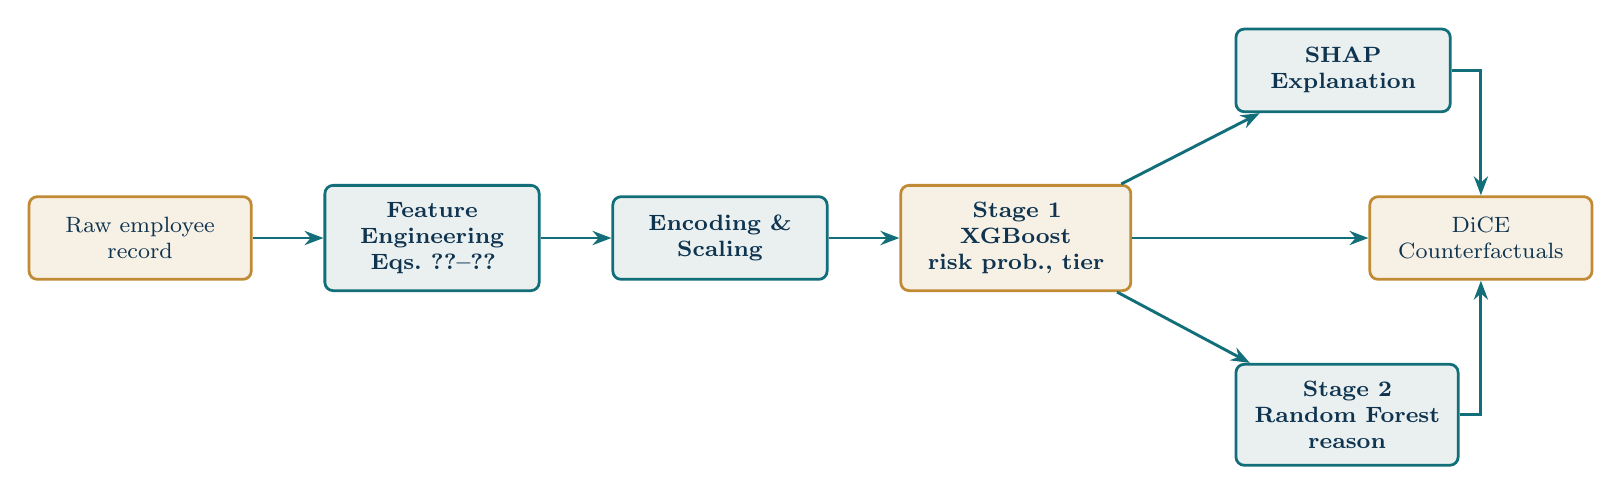
\begin{tikzpicture}[node distance=0.9cm]
  \node[data,text width=2.4cm] (in) {Raw employee\\record};
  \node[stage,text width=2.3cm,right=of in] (fe) {Feature\\Engineering\\\footnotesize Eqs.\ \ref{eq:income}--\ref{eq:satisfaction}};
  \node[stage,text width=2.3cm,right=of fe] (pre) {Encoding \&\\Scaling};
  \node[stage,text width=2.5cm,right=of pre,fill=TPlightgold,draw=TPgold] (s1) {Stage 1\\XGBoost\\\footnotesize risk prob., tier};
  \node[stage,text width=2.3cm,above right=0.9cm and 1.3cm of s1,fill=TPlight] (shap) {SHAP\\Explanation};
  \node[stage,text width=2.4cm,below right=0.9cm and 1.3cm of s1,fill=TPlight] (s2) {Stage 2\\Random Forest\\\footnotesize reason};
  \node[data,text width=2.4cm,right=3.0cm of s1,fill=TPlightgold] (dice) {DiCE\\Counterfactuals};
  \draw[fl] (in)--(fe); \draw[fl] (fe)--(pre); \draw[fl] (pre)--(s1);
  \draw[fl] (s1)--(shap); \draw[fl] (s1)--(s2);
  \draw[fl] (s1) -- (dice.west);
  \draw[fl] (shap.east) -| (dice.north);
  \draw[fl] (s2.east) -| (dice.south);
\end{tikzpicture}}
\caption{Module 3 two-stage architecture. Stage 1 (XGBoost) predicts risk; SHAP explains that prediction; Stage 2 (Random Forest) predicts the most likely reason, for at-risk employees; DiCE combines both to propose counterfactual interventions.}
\label{fig:mod3-pipeline}
\end{figure}

\subsection{Stage 1: XGBoost Attrition Risk Model}

This subsection specifies the primary risk-classification model, discussing algorithm formulation, hyperparameter optimization, calibrated risk tiers, and comparative benchmark performance.

\subsubsection{Algorithm}

XGBoost (Extreme Gradient Boosting, Chen and Guestrin, 2016) builds a regularized additive ensemble of decision trees, where each new tree is fit to the negative gradient of the loss with respect to the current ensemble's predictions. For a dataset of $n$ examples, the model's training objective at boosting round $t$ is

\begin{formulabox}
\begin{equation}
\label{eq:xgb-obj}
\mathcal{L}^{(t)} = \sum_{i=1}^{n} l\big(y_i,\ \hat{y}_i^{(t-1)} + f_t(\mathbf{x}_i)\big) \;+\; \Omega(f_t), \qquad \Omega(f) = \gamma T + \tfrac{1}{2}\lambda \lVert w \rVert^2
\end{equation}
\end{formulabox}

where $f_t$ is the tree added at round $t$, $l$ is a differentiable loss (log loss, for this binary classification task), and $\Omega$ regularizes tree complexity directly, with $T$ the number of leaves and $w$ the leaf weight vector, discouraging both overly large trees and overly large leaf values. XGBoost was selected over alternatives for this dataset because it handles missing values natively, integrates \code{scale\_pos\_weight} to directly counterbalance class imbalance, captures non-linear feature interactions (relevant given the deliberately interactive \code{burnout\_proxy} feature of Equation~\ref{eq:burnout}), integrates natively with SHAP for exact, efficient explainability, and performs strongly on tabular data at this sample scale.

\subsubsection{Hyperparameters and Risk Tiers}

\begin{table}[H]
\centering
\caption{Stage 1 XGBoost hyperparameters}
\label{tab:mod3-hyperparams}
\small
\begin{tabular}{p{3.4cm}p{2.2cm}p{8.2cm}}
\toprule
\hdrow \hdtxt{Hyperparameter} & \hdtxt{Value} & \hdtxt{Rationale} \\
\midrule
\code{n\_estimators} & 500 & Sufficient tree count for convergence \\
\rowcolor{TPlight}
\code{max\_depth} & 5 & Controls model complexity; limits overfitting \\
\code{learning\_rate} & 0.05 & Low rate with a larger tree count for better generalization \\
\rowcolor{TPlight}
\code{subsample} & 0.8 & Row-level bagging; reduces variance \\
\code{colsample\_bytree} & 0.8 & Column-level bagging; reduces tree correlation \\
\rowcolor{TPlight}
\code{scale\_pos\_weight} & $\approx 5.2$ & Ratio of majority to minority class ($1233/237$) \\
\code{min\_child\_weight} & 3 & Minimum leaf weight; regularizes noisy splits \\
\rowcolor{TPlight}
\code{eval\_metric} & \code{auc} & Directly optimizes the metric that matters for imbalanced data \\
\code{tree\_method} & \code{hist} & Histogram-based split finding; faster, memory-efficient \\
\bottomrule
\end{tabular}
\end{table}

The continuous risk probability output by Stage 1 is mapped to one of four operational risk tiers, shown in Table~\ref{tab:mod3-tiers}, that drive the visual and workflow treatment an employee receives in the application described in Section~\ref{sec:frontend}.

\begin{table}[H]
\centering
\caption{Attrition risk tier thresholds}
\label{tab:mod3-tiers}
\small
\begin{tabular}{llp{7.5cm}}
\toprule
\hdrow \hdtxt{Probability range} & \hdtxt{Tier} & \hdtxt{Interpretation} \\
\midrule
0.00 -- 0.29 & Low & Stable; no immediate action needed \\
\rowcolor{TPlight}
0.30 -- 0.49 & Medium & Early warning; monitor and check in \\
0.50 -- 0.69 & High & Significant risk; HR intervention recommended \\
\rowcolor{TPlight}
0.70 -- 1.00 & Critical & Imminent flight risk; immediate escalation \\
\bottomrule
\end{tabular}
\end{table}

\subsubsection{Results and Comparison with LightGBM}

\begin{table}[H]
\centering
\caption{Stage 1 test-set results, and comparison against a LightGBM baseline}
\label{tab:mod3-results}
\small
\begin{tabular}{C{2.8cm}C{2.3cm}C{2.0cm}p{6.4cm}}
\toprule
\hdrow \hdtxt{Metric} & \hdtxt{XGBoost (chosen)} & \hdtxt{LightGBM} & \hdtxt{Assessment} \\
\midrule
Accuracy & 84.01\% & 84.01\% & Misleading; dominated by the majority class \\
\rowcolor{TPlight}
AUC-ROC & \textbf{80.14\%} & 77.24\% & Primary metric; well above the 50\% random baseline \\
F1 (macro) & 69.98\% & --- & Balanced across both classes \\
\rowcolor{TPlight}
F1 (minority class) & 49.46\% & 47.19\% & Moderate; catches roughly half of true leavers \\
Precision (minority) & 50.00\% & --- & Half of flagged employees are genuinely at risk \\
\rowcolor{TPlight}
Recall (minority) & 48.94\% & --- & Roughly half of true at-risk employees are caught \\
\bottomrule
\end{tabular}
\end{table}

An AUC-ROC of 0.8014 means that, given one randomly chosen employee who actually left and one who stayed, the model assigns the higher risk score to the one who left 80.14\% of the time, a substantial and genuinely useful discriminative signal for a real-world HR dataset of this size. XGBoost outperforms a comparably tuned LightGBM baseline by 2.9 AUC points and was selected on that basis. The minority-class F1 of 49.46\% is reported here without inflation: of every 100 employees who would genuinely leave, the model correctly flags approximately 49, at a cost of roughly one false alarm for every true positive caught. This is treated candidly as the model's most important limitation, discussed further in Section~\ref{sec:mod3-limits}, rather than presented as a stronger result than it is; the counterbalancing fact, also stated plainly, is that catching even half of departures proactively is a substantial improvement over catching none, and that the asymmetric cost of a false positive (an unnecessary but low-cost HR conversation) against a false negative (the loss of a valuable employee) makes this operating point defensible even without further tuning.

\subsection{Stage 2: Random Forest Reason Classifier}

For any employee flagged at risk by Stage 1, a second classifier predicts the most likely underlying reason among four categories: \emph{Burnout} (driven by overtime, poor work-life balance, low satisfaction), \emph{Compensation} (income significantly below departmental peers), \emph{Stagnation} (long tenure without promotion), and \emph{Career Growth} (high ambition in a role offering limited advancement). Because the IBM dataset contains no ground-truth ``reason'' field, training labels for \code{Attrition=Yes} employees are assigned by rule-based heuristics, for example \emph{Burnout} when \code{burnout\_proxy} exceeds a threshold or (\code{OverTime=Yes} and \code{WorkLifeBalance} $\leq 2$), and \emph{Compensation} when \code{income\_to\_dept\_avg} $< 0.85$; this is stated explicitly as a known limitation, since these labels are synthetic rather than drawn from real exit-interview data. A \code{RandomForestClassifier} (\code{n\_estimators=200}, \code{max\_depth=6}, \code{class\_weight='balanced'}) was chosen for this stage because it handles multi-class output natively with calibrated probability estimates, resists overfitting on the smaller Yes-only training subset, and provides a full probability distribution over all four reasons rather than a single hard label.

The reported 95.74\% accuracy on this stage should be read cautiously: because training labels are derived from the same underlying features via fixed rules, the Random Forest partially re-learns those rules rather than demonstrating independent generalization to unseen ground truth. The macro F1 of 65.83\% across four classes (against a 25\% random baseline) is the more informative figure, and Stage 2's output is positioned throughout this report, and in the deployed application, as an \emph{HR hypothesis generator}, pointing toward the most probable contributing factor to guide a targeted conversation, not as a definitive diagnosis.

\subsection{SHAP: Per-Employee Explainability}
\label{sec:mod3-shap}

This subsection details the game-theoretic SHAP interpretability framework employed to explain individual attrition risk predictions through localized feature attributions.

\subsubsection{Theoretical Background}

SHAP (SHapley Additive exPlanations; Lundberg and Lee, 2017) grounds feature attribution in cooperative game theory. Treating the $|F|$ input features as players in a cooperative game whose payoff is the model's prediction, the Shapley value for feature $i$ is the average marginal contribution of that feature across every possible ordering in which features could be revealed to the model:

\begin{formulabox}
\begin{equation}
\label{eq:shapley}
\varphi_i \;=\; \sum_{S \subseteq F \setminus \{i\}} \frac{|S|!\,(|F|-|S|-1)!}{|F|!} \Big[ f\big(S \cup \{i\}\big) - f(S) \Big]
\end{equation}
\end{formulabox}

where $f(S)$ is the model's expected output conditioned on knowing only the features in subset $S$. This construction is the unique attribution scheme satisfying four game-theoretic fairness axioms (efficiency, symmetry, dummy, and additivity) simultaneously, and it guarantees the additive decomposition used throughout this section and the deployed application:

\begin{formulabox}
\begin{equation}
\label{eq:shap-additive}
f(\mathbf{x}) \;=\; \phi_0 \;+\; \sum_{i=1}^{|F|} \varphi_i(\mathbf{x})
\end{equation}
\end{formulabox}

where $\phi_0$ is the model's base value (its expected output over the training distribution) and each $\varphi_i$ is that specific prediction's exact contribution from feature $i$. A positive $\varphi_i$ increases the predicted attrition probability relative to the base rate (a risk factor); a negative $\varphi_i$ decreases it (a protective factor).

\subsubsection{Implementation}

Exhaustively enumerating Equation~\ref{eq:shapley} over all feature subsets is intractable for more than a handful of features, but for tree-based models such as XGBoost, the exact Shapley values can be computed efficiently via \code{shap.TreeExplainer}, which exploits the tree structure directly rather than approximating. The measured base value for the deployed Stage 1 model is $\phi_0 = 1.401708$ in log-odds space, which converts through the sigmoid function to $\sigma(\phi_0) = e^{\phi_0}/(1+e^{\phi_0}) \approx 0.80$ in probability space, consistent with the approximately 80--84\% majority-class rate in the training data.

The additive property of Equation~\ref{eq:shap-additive} is also used as a direct correctness check on the explanation itself, not just accepted on faith: for every scored employee, the base value plus the sum of that employee's SHAP values is compared against the model's actual predicted probability for them, and the discrepancy is required to stay below $0.001$. This is a mathematical consistency check rather than a measure of predictive quality, but it confirms that the numbers shown to an HR administrator as ``why this score'' genuinely do sum to the score itself, rather than being a plausible-looking approximation.

\subsubsection{Global and Local Results}

Averaged across the full dataset, the mean absolute SHAP value of the single most influential feature, \code{JobSatisfaction}, is $0.6628$, against a mean absolute SHAP value of $0.3169$ across all features globally, meaning \code{JobSatisfaction} carries roughly twice the average feature's explanatory power and is confirmed as the dominant global driver, consistent with organizational-behaviour research that consistently identifies job satisfaction as a leading predictor of voluntary turnover. All four engineered features from Section~\ref{sec:mod3-features} appear among the top five most frequently top-ranked features across the employee population, directly validating the feature-engineering effort rather than relying on assumption alone. Beyond this global view, SHAP additionally provides a fully personalized, per-employee explanation: for any individual, the top five features by absolute SHAP value, together with their sign, are surfaced as ``Key Risk Drivers'' in the deployed application.

\subsection{DiCE: Counterfactual Intervention Engine}
\label{sec:mod3-dice}

This subsection outlines the counterfactual optimization framework used to formulate actionable, minimum-perturbation intervention plans that demonstrably lower an employee's predicted attrition risk.

\subsubsection{Theoretical Background}

Diverse Counterfactual Explanations (DiCE; Mothilal, Sharma, and Tan, 2020) frames actionable explanation as an optimization problem: given a model $f$ and an instance $x$ with an undesired predicted outcome, find a nearby instance $x'$ (or a diverse set of such instances) for which $f(x')$ crosses a desired decision boundary, while minimizing the distance travelled from $x$ and restricting changes to features that are actually mutable in practice. In its general form, this is posed as minimizing a loss combining outcome achievement, proximity, and a diversity term across a requested set of counterfactuals.

\subsubsection{Implementation in TalentPulse}

Rather than deploying the general DiCE optimization library directly, TalentPulse implements a custom, constrained single- and paired-feature perturbation engine that mirrors DiCE's objective while remaining fully deterministic and directly interpretable for HR use. Table~\ref{tab:mod3-mutable} lists the mutable features the engine is permitted to search over; every other feature (age, gender, tenure, and so on) is held fixed, since they are not levers HR can actually pull.

\begin{table}[H]
\centering
\caption{Mutable features available to the DiCE-style intervention engine}
\label{tab:mod3-mutable}
\small
\begin{tabular}{p{3.6cm}p{2.6cm}p{7.2cm}}
\toprule
\hdrow \hdtxt{Feature} & \hdtxt{Type} & \hdtxt{Candidate values} \\
\midrule
OverTime & Binary & Remove overtime only \\
\rowcolor{TPlight}
JobSatisfaction & Ordinal 1--4 & Higher values only \\
EnvironmentSatisfaction & Ordinal 1--4 & Higher values only \\
\rowcolor{TPlight}
WorkLifeBalance & Ordinal 1--4 & Higher values only \\
StockOptionLevel & Ordinal 0--3 & Higher values only \\
\rowcolor{TPlight}
JobLevel & Ordinal 1--5 & Higher values only \\
YearsSinceLastPromotion & Ordinal & Lower values only (simulated promotion) \\
\rowcolor{TPlight}
TrainingTimesLastYear & Discrete & Higher of $\{2,3,4,5,6\}$ \\
MonthlyIncome & Continuous & $+10\%$, $+20\%$, $+30\%$ of current \\
\rowcolor{TPlight}
DistanceFromHome & Continuous & Set to 1 (simulated remote/hybrid work) \\
\bottomrule
\end{tabular}
\end{table}

For a given employee, the engine generates three candidate plans: \textbf{CF1}, the single (feature, value) change from Table~\ref{tab:mod3-mutable} that produces the greatest risk reduction, subject to that reduction exceeding a 0.5\% minimum threshold; \textbf{CF2}, the second-largest single-feature reduction using a \emph{different} feature from CF1, ensuring the two alternatives are genuinely diverse rather than trivial variations of the same lever; and \textbf{CF3}, the combined application of the CF1 and CF2 features simultaneously, modelling the synergistic effect of a combined HR strategy rather than assuming the individual effects simply add. Critically, every reported predicted risk figure is not the counterfactual generator's own internal estimate; it is re-verified by literally applying the proposed change to a copy of the employee's real feature vector and re-running the trained Stage 1 model on the result, so the number shown to an HR administrator and the number produced by actually clicking ``Apply'' in the application are guaranteed to be the same figure.

\subsubsection{Results}

Across the dataset, the average absolute risk reduction achieved per counterfactual set is $36.12$ percentage points, and $233$ employees, approximately $16\%$ of the full population, closely tracking the dataset's own $16.1\%$ attrition rate, received at least one valid intervention exceeding the minimum threshold. For an employee at $0.85$ attrition probability, the best single intervention typically reduces risk to approximately $0.85 - 0.36 = 0.49$, moving them from the Critical to the Medium tier. Employees who receive no valid intervention typically have every mutable feature already at its optimal value, or have a prediction driven predominantly by immutable features such as age or number of prior employers, for which no lever in Table~\ref{tab:mod3-mutable} applies. The CF3 combined plan consistently outperforms CF1 or CF2 in isolation, directly demonstrating the practical value of combined retention strategies over single-lever interventions; the single most powerful individual intervention across the dataset is typically improving job satisfaction where it is currently low, or reducing commute distance as a proxy for offering remote or hybrid work.

What this engine has not been shown to do, and what this report states plainly rather than glosses over, is prove that any of these interventions actually reduce attrition once applied to a real employee. What is validated is internal consistency: that a proposed change is achievable within the constraints of Table~\ref{tab:mod3-mutable}, and that re-running the trained model on the changed record produces the risk reduction reported. Establishing that the intervention causes a real reduction in the chance someone leaves would require a randomized controlled trial inside an actual company: assigning comparable at-risk employees to a control group and an intervention group, applying the change for real, and waiting six to twelve months to observe who actually stays. That kind of trial needs an industry partner, employee consent, and ethical approval, none of which are available within the scope of this capstone, so the DiCE engine's output is best understood as a well-grounded hypothesis for HR to act on, not a proven causal guarantee, and that gap is documented here as future work rather than left unstated.

Module 3 was also designed to optionally accept a fifth, cross-module feature, a skill-gap score expressing what fraction of a role's required skills an employee is missing, supplied by Module 2. This was planned as a controlled experiment: retrain the model with the 31 features already listed plus this one additional signal, and check whether it measurably improves accuracy or AUC-ROC over the baseline. That cross-module retraining pass was not carried out; the model documented throughout this section is the 31-feature baseline, trained and evaluated entirely on the IBM HR Analytics dataset without any dependency on Module 2's output. The skill-gap integration remains a defined, reasonable next step rather than a component of the shipped system.

\subsubsection{Worked Example}

Table~\ref{tab:mod3-example} traces one complete, real prediction end to end for an illustrative employee: a 41-year-old Sales Executive earning \$5{,}993 per month, working overtime, with a work-life balance score of 1 and an environment satisfaction score of 2.

\begin{table}[H]
\centering
\caption{End-to-end worked example}
\label{tab:mod3-example}
\small
\begin{tabular}{p{4.4cm}p{8.0cm}}
\toprule
\hdrow \hdtxt{Stage} & \hdtxt{Output} \\
\midrule
Stage 1 (risk) & Attrition probability $= 0.9833$ (98.33\%), risk tier \textbf{Critical} \\
\rowcolor{TPlight}
Top SHAP factor & JobSatisfaction $=4 \Rightarrow \varphi = -1.276$ (protective) \\
2nd SHAP factor & burnout\_proxy $=3 \Rightarrow \varphi = +1.136$ (strongly increases risk) \\
\rowcolor{TPlight}
3rd SHAP factor & WorkLifeBalance $=1 \Rightarrow \varphi = +0.930$ (increases risk) \\
Stage 2 (reason) & \textbf{Burnout}, 89\% confidence \\
\rowcolor{TPlight}
CF1 & Improve work-life balance $1 \to 4$: probability drops to 0.9217 ($-6.15$ pts) \\
CF2 & Grant stock options $0 \to 1$: probability drops to 0.9482 ($-3.51$ pts) \\
\rowcolor{TPlight}
CF3 (combined) & Both changes together: probability drops to 0.8520 ($-13.13$ pts) \\
\bottomrule
\end{tabular}
\end{table}

Even the best combined intervention available leaves this particular employee at a still-high 85.2\% predicted risk, correctly signalling to HR that this is a genuinely difficult retention case, driven overwhelmingly by burnout, that would require immediate workload relief and a direct, honest career conversation rather than a single low-effort fix.

\subsection{Results Analysis, Strengths, and Limitations}
\label{sec:mod3-limits}

Table~\ref{tab:mod3-strengths} summarizes Module 3's strengths and limitations together, as a matched pair, since an honest account of applied machine learning results requires reporting both.

\begin{table}[H]
\centering
\caption{Module 3: strengths and limitations, reported together}
\label{tab:mod3-strengths}
\small
\begin{tabular}{p{6.6cm}p{6.6cm}}
\toprule
\hdrow \hdtxt{Strengths} & \hdtxt{Limitations} \\
\midrule
AUC-ROC (80.14\%) chosen deliberately over accuracy for imbalanced data & Dataset is small (1{,}470 records); minority-class F1 is approximately 50\% \\
\rowcolor{TPlight}
All four engineered features rank in the global top five by SHAP importance & Stage 2 reason labels are rule-derived, not ground-truth exit-interview data \\
Dual-model design cleanly separates risk detection from reason explanation & Minority-class recall ($\approx 49\%$) misses roughly half of true leavers \\
\rowcolor{TPlight}
Every prediction carries a full, exact, per-employee SHAP explanation & CF1/CF2 search only single features; higher-order synergy is only captured by CF3's fixed pairing \\
DiCE-style interventions are specific, actionable, and re-verified, not estimated & Fixed salary-increment steps are not benchmarked against real market data \\
\rowcolor{TPlight}
No training-serving skew; the preprocessor is serialized and reused identically at inference & No temporal or trend features (engagement history, recency) are captured \\
\bottomrule
\end{tabular}
\end{table}

Documented directions for future improvement, in order of expected impact, include collecting substantially more labelled data (the dataset's 1{,}470 records is judged the single largest bottleneck on minority-class recall), tuning the decision threshold from the default $0.50$ toward $0.35$--$0.40$ to trade some precision for materially better recall, applying SMOTE or a related oversampling technique to the training minority class, incorporating additional features such as engagement-survey trends, one-on-one meeting frequency, and manager-change history, and adopting k-fold cross-validation for a more robust evaluation given the dataset's modest size.

\subsection{API Architecture}

Module 3 is served as a FastAPI application (\code{GET /}, \code{GET /employees}, \code{GET /employees/\{id\}}, \code{POST /infer}, \code{GET /infer/\{id\}}), with all four model artefacts (the Stage 1 XGBoost model, the Stage 2 Random Forest model, the fitted preprocessor, and the ordered feature-column list) loaded once at container startup, and the SHAP \code{TreeExplainer} constructed once at that same startup to avoid repeated initialization overhead on every request. A single inference call returns the complete response contract used throughout Section~\ref{sec:frontend}, comprising the attrition probability and verdict, the risk tier, the Stage 2 reason distribution, the SHAP base value and top-five attributions, and the full set of DiCE-style intervention plans, in one payload.

\clearpage
%============================================================================
\section{Technology Stack}
\label{sec:techstack}

Table~\ref{tab:full-stack} consolidates the complete technology stack of the deployed system across every layer, extending the architectural summary of Section~\ref{sec:arch} with implementation-level detail.

\begin{table}[H]
\centering
\caption{Complete technology stack, as deployed}
\label{tab:full-stack}
\small
\begin{tabular}{p{2.8cm}p{4.6cm}p{6.6cm}}
\toprule
\hdrow \hdtxt{Layer} & \hdtxt{Technology} & \hdtxt{Notes} \\
\midrule
Frontend framework & React 19, Vite 7 & Single-page application \\
\rowcolor{TPlight}
Styling & Tailwind CSS 4 & Utility-first styling, dark/light theming \\
Motion & Framer Motion & UI transitions and micro-interactions \\
\rowcolor{TPlight}
Backend runtime & Node.js, Express 5 & Application logic, authentication proxy, single ML-call boundary \\
Database & MongoDB Atlas (Mongoose ODM) & Document store for applications, employees, screening runs, learning paths \\
\rowcolor{TPlight}
File storage & MongoDB GridFS & Stores uploaded CV files with a metadata sidecar collection \\
Authentication & Clerk & Additive role model: applicant, employee, admin on one identity \\
\rowcolor{TPlight}
Module 1a service & Python, FastAPI, GLiNER & Skill extraction, resume and job-description text \\
Module 1b service & Python, FastAPI, Sentence-Transformers, PyTorch & Resume-JD ranking and adversarial debiasing \\
\rowcolor{TPlight}
Module 2 service & Python, FastAPI, GLiNER, Sentence-Transformers, NetworkX & Skill-gap analysis and course recommendation \\
Module 3 service & Python, FastAPI, XGBoost, scikit-learn, SHAP & Attrition prediction, explanation, and intervention generation \\
\rowcolor{TPlight}
Frontend hosting & Vercel & Static build and serverless function hosting \\
ML hosting & Hugging Face Spaces (Docker SDK) & Four independently deployed containers, one per inference service \\
\bottomrule
\end{tabular}
\end{table}

Every machine-learning capability described in Sections~\ref{sec:mod1}--\ref{sec:mod3} is served over a real HTTP call to one of these four independently hosted services; none of the model behaviour described in this report is mocked or simulated in the deployed application, a distinction verified directly against the running system and documented further in Section~\ref{sec:frontend-honest}.

\clearpage
%============================================================================
\section[Frontend Application Workflow]{Frontend Application and End-to-End Workflow}
\label{sec:frontend}

This section walks through the complete TalentPulse web application deployed on Vercel. We follow the practical workflows from both perspectives: job applicants submitting resumes and monitoring application status, and HR administrators managing postings, evaluating candidates with debiased screening, planning structured employee training, and mitigating attrition risk. All descriptions reflect the exact, live behavior of the production platform.

\subsection{Identity and the Additive Role Model}

A single Clerk-authenticated identity in TalentPulse can simultaneously hold any combination of three roles: \emph{applicant}, \emph{employee}, and \emph{admin}. Roles are additive rather than exclusive; being hired grants an employee role alongside, not instead of, an existing applicant role, which is precisely why a real, recruited employee can browse and apply for a different internal opening from the exact same account used to review their own attrition score, and why an HR administrator's own account can be used to exercise the applicant-facing flow without a second login. A ``Switch workspace'' control in the top-right menu changes which interface renders for the currently signed-in user; it is a view change, not a re-authentication.

\subsection{Dashboard}

The administrator's landing page surfaces the headline ``People at risk of leaving'' figure, a risk-distribution chart, and stat tiles for headcount, open roles, new applications, and shortlisted candidates, all computed from real, live collections rather than placeholder values; the at-risk list and its distribution chart read directly from the \code{predictions} collection that Module 3 writes to every time it scores an employee, so this page functions as a summary view rather than a duplicate calculation path. Clicking into any entry on the at-risk list navigates directly to that specific employee's detail page in the Employees module.

\subsection{Recruitment: From Posting a Job to a Hiring Decision}

An administrator posts a job with a title, department, location, and a job description of at least 40 characters; required skills are then extracted automatically via the Module 1 skill-extraction service (Section~\ref{sec:mod1-skillex}) and rendered as removable chips once extraction completes. Once published, the posting accepts applications; each submitted resume is processed by two independent pathways simultaneously, for two different purposes. The skill and match-quality pathway stores the file in GridFS, extracts categorized skills via the same skill extractor used for job descriptions, and computes an immediate heuristic skill-overlap score shown to the applicant on their own submission; the heavier, genuinely ML-driven semantic ranking against the specific posting (Section~\ref{sec:mod1-model}) only runs when an administrator explicitly opens the Fair-Screen report, since it is a comparatively expensive operation not suited to running on every single submission. The demographic pathway runs \code{biasExtractor.js} (Section~\ref{sec:mod1-skillex}) independently over the same document. A cooldown, 24 hours by default and configurable per posting, prevents the same account from submitting repeated applications to the same job in immediate succession.

Invoking ``Fair-Screen Candidates'' on a posting with applicants produces the full ten-stage report detailed in Table~\ref{tab:mod1-report}, culminating in a shortlist decision interface with Shortlist, Reject, and Undo controls per candidate, alongside the debiased model's own recommended score bands, which remain a recommendation rather than an enforced rule; an administrator can shortlist a candidate the model would have rejected, or the reverse. On a posting with shortlisted candidates, ``Recruit from Shortlisted'' opens the final, deliberately separate hiring decision: \emph{Recruit} creates a real employee record (initialized with neutral, day-one placeholder values for fields Module 3 needs but that a five-minute-old hire cannot yet genuinely have, such as tenure and satisfaction survey scores) and grants the employee role on the candidate's linked account in one step, while \emph{Do Not Recruit} requires an internal, admin-only reason that is never surfaced to the candidate, who sees only that they were not selected. Recruiting no longer assumes the candidate must join the posting's own department: an inline picker in the same modal asks the administrator to choose between the posting's own department (matched case-insensitively against departments already on file, so a posting filed under ``cse'' joins the existing ``CSE'' rather than quietly forking a near-duplicate), any other existing department drawn from the live employee roster, or a freshly typed new one, since Department is a free-text field on the Employee record rather than a table of its own and so ``creating'' one is simply hiring its first member. The success message names the destination department directly, and that department, not necessarily the posting's, is what gets stamped onto the new employee record and onto the application's own history. Either decision removes that candidate from every live view of that specific posting, since the hiring stage is complete for them either way, which is distinct from a screening-stage rejection, after which a candidate remains visible since fair-screening and final recruitment are treated as genuinely separate decisions.

A posting whose deadline has passed is not a dead end. Its action button changes to ``Reopen,'' which prompts for a new deadline (required, and rejected server-side if it is not genuinely in the future) and, once confirmed, flips the posting back to accepting applications under the new date. A posting an administrator stopped manually, rather than one that expired on its own, reopens the same way without the deadline prompt, since its deadline was never actually the reason it stopped accepting applications.

\subsection{Employees: The Retention Module}

Opening any employee who has been scored at least once by Module 3 surfaces three elements in sequence: the attrition risk percentage itself, labelled against the company baseline (approximately 16\%) and bucketed into the risk tiers of Table~\ref{tab:mod3-tiers}, together with the Stage 2 primary predicted reason and its confidence; the top-five SHAP ``Key Risk Drivers'' for that specific individual (Section~\ref{sec:mod3-shap}); and two to three DiCE-style ``Intervention Plans'' (Section~\ref{sec:mod3-dice}), each naming one or two concrete changes together with the model's predicted post-change risk. \emph{Apply} writes the proposed change to the employee's real record and re-runs the model once on the result, so a whole plan moves together rather than one field at a time; \emph{Undo} reverses the most recent change (and can itself be reversed, chaining correctly back through history); and \emph{Re-run model} forces a fresh inference call rather than serving a cached score, useful immediately after an administrator has manually corrected an employee's details.

\subsection{Upskilling and Job Match}

The Upskilling module runs Module 2 (Section~\ref{sec:mod2}) for a chosen target role, either an existing posting or a freshly typed description, against either a single selected employee or, in Cohort mode, several at once with shared-course consolidation across the group. Below the resulting course plan, a cost-effectiveness breakdown, computed by the Express backend rather than the ML service itself since it depends on the employee's actual salary and the posting's actual salary range, reports training cost and hours, an assumed ramp-up cost for settling into a new role, and, where a posting's salary range makes it possible, a salary payback period estimating how many months of increased income it would take to recoup the training investment. A ``Recommend this learning path'' control saves the generated plan directly into the employee's own record, fires a notification, and makes it visible in that employee's own portal, functioning only for employees with a genuine linked account. Job Match inverts the direction: starting from a job rather than a person, it pre-filters the entire employee base for free using simple skill-overlap counting, then runs the genuine Module 2 scoring pipeline only on the resulting top-N candidates, since scoring the full employee base with the real model would be prohibitively slow. Its composite ranking score deliberately weights skill readiness at 60\%, the employee's own current attrition risk at 25\%, and performance rating at 15\%, a design decision that makes Job Match quietly a retention tool as well as a hiring tool, since a good skill match who is already at meaningfully elevated attrition risk is intentionally promoted up the ranking, on the reasoning that an internal move is itself a genuine retention lever.

\subsection{Onboarding and the CV Library}

Clerk owns the sign-up form itself, email and password, and offers no way to embed a file picker inside it, so everything else an application needs is collected immediately afterward, in a short one-time onboarding step: profile details first (name, phone, location, headline, years of experience, and optional LinkedIn and portfolio links), then a CV library. Every CV picked here uploads and is parsed by the Module 1 skill extractor the moment it is selected, one file per request rather than batched, since batching several uploads into a single call is how a cold, serverless model space is made to hit its own timeout, and one slow document should not stall the others. Both the profile and the CV list are written to the database as they are entered rather than held until a final submit, so nothing is lost if the tab closes partway through. Applying to a job later is then only a choice from an already-parsed list rather than a fresh upload; the same CV Library component reappears, unchanged, inside the applicant's own profile tab for adding or retiring CVs at any later time, and inside the apply modal itself for anyone who arrives at a posting without having onboarded a CV yet.

\subsection{Applicant and Employee Portals}

The Applicant Portal lists open roles, supports applying with an attached resume and an optional role-specific cover letter, and shows every submitted application's current status together with a full timeline of status changes, never exposing the internal reasoning behind a decline. The Employee Portal mirrors the administrator's own Employees view but scoped to the signed-in employee, presenting their own risk reading in softer, first-person framing, the same SHAP-derived factors reframed as ``What's shaping this,'' and the same DiCE-style interventions reframed as ``Suggested conversations'' for a manager one-on-one rather than buttons an administrator clicks directly. A compact ``Learning paths'' summary card expands into a full panel of every path an administrator has recommended, visually distinguishing unread entries, and a ``Looking for an internal move'' banner links back into the same account's applicant view, closing the loop the additive role model exists to support.

\subsection{People and Roles}

A separate People and Roles screen, visible only to administrators, is where the additive identity model of Section~\ref{sec:frontend} is actually managed. Every account starts as an applicant the moment someone signs in for the first time; granting a role adds a badge next to that account rather than replacing whatever badges are already there, so one row in this view can carry Applicant, Employee, and Admin badges on the same person at once, with a linked employee number shown next to the Employee badge when it applies. Revoking the employee role does not delete that employee's history: their record is marked \code{former} rather than erased, which is what allows the re-application history described below to still find it later.

\subsection{Notifications and Search}

A bell icon in the top bar fires on every state change that matters to whoever is signed in: a new application arriving, a fair-screen run finishing, a status change on any of an applicant's own submissions, being recruited or declined, a learning path being recommended, and a real, measured drop in attrition risk after an intervention is applied. Clicking a notification jumps straight to whatever it concerns rather than only marking it read. A separate command-palette search, opened with Cmd+K or by clicking the header's search box, jumps to any sidebar section or any person, employee or applicant, matched by name; it reads the same data every other screen already reads rather than maintaining its own separate index. Every page that has its own search or filter box, Employees, Recruitment, Upskilling, and People and Roles among them, keeps that box's typed text local to that page, so switching pages and back never leaves a stale filter applied.

\subsection{Ending an Employment and Re-Application History}

Two mirrored paths end an employment record, and TalentPulse deliberately remembers which one was used. From the Employees view, an administrator can remove an active employee, providing a short reason inline; from the Employee Portal, an employee can end their own record the same way, through a ``Looking to leave?'' banner that keeps their applicant access intact on the same account. Both paths flip the underlying record to \code{former}, dated, with the reason on file, but they are stored as two distinct facts rather than one, an admin-initiated removal and a self-initiated departure, because who ended an employment and why are genuinely different things to know about a person later, even though both end in the same status.

That distinction resurfaces if the same identity ever applies again, to any job, at any later point. Their application card then carries a real employment-history line, department, exit date, and reason, drawn directly from the employee record that ended, not reconstructed or guessed; and because a person can genuinely be hired, leave, and be rehired more than once, every past stint is listed if there is more than one, not only the most recent. A related consolidation was made deliberately: since being recruited already implies having cleared the shortlist stage, a returning, previously recruited candidate shows a single ``Current employee'' tag rather than that tag sitting alongside a redundant ``Previously shortlisted'' badge that says the same thing a second way, and their own history entry for that recruitment reads ``Joined as [role] in [department] on [date]'' rather than ``Recruited,'' since from inside their own timeline it is the day they joined, not a decision someone else made about them; the department named is the one they were actually placed into at recruiting time, which is not always the posting's own department now that an administrator can choose otherwise.

\subsection{Real Defects Found and Fixed While Testing}

A short account of what actually broke during development is worth keeping here, both for the record and because it reflects the depth of testing this system went through rather than a system exercised only in the abstract. A former employee could appear on the Dashboard's ``highest attrition risk'' list, since someone who has already left cannot meaningfully be described as at risk of leaving, and clicking their name used to dead-end rather than open a real profile; the leaderboard now only draws from active employees. A candidate's card on a second, unrelated job posting used to keep showing a stale outcome (``shortlisted,'' say) for weeks after they had actually been recruited or declined on a different posting entirely, because that summary line was written once at submission time and never revisited; it now refreshes the moment any final decision lands on any of that person's applications. The fair-screening report's own candidate count used to silently include someone who already had a final recruit-or-decline decision on file, so a job showing ``2 applicants'' on its card could still fair-screen three people; the ranking route now applies the exact same filter the visible applicant list already used. And the department filters in Job Match and Upskilling used to build their dropdown only from departments that already had employees in them, so a department that existed only because a job posting had just named it would not appear as a filterable option until someone was actually hired into it; both dropdowns now also read department names directly off job postings.

\subsection{What Is Real, and What Is Documented Simulation}
\label{sec:frontend-honest}

In the interest of the same technical honesty applied throughout this report, one boundary is stated explicitly here rather than left implicit. Skill extraction, semantic ranking and debiasing, gap analysis and learning-path generation, and attrition scoring with SHAP and DiCE are all genuine, live HTTP calls to the four independently hosted services of Section~\ref{sec:techstack}, verified directly against the running system rather than assumed from source code. The one deliberately simulated element in the entire pipeline is the skin-colour field consumed by Module 1's debiasing model, which, as documented in Section~\ref{sec:mod1-skillex}, requires an explicit statement no real resume would ever contain and exists purely so a model trained expecting that feature has a defined value to reason about; every other demographic and skill signal used throughout the system is extracted from genuine, unmodified document text.

\clearpage
%============================================================================
\section{Application Screenshots}
\label{sec:screenshots}

This section presents screenshots of the deployed TalentPulse platform across its primary user workflows, captured directly from the live Vercel deployment.

%------------------------------------------------------------
\subsection{Authentication and Account Setup}

TalentPulse uses Clerk authentication with an additive role structure. Users register as applicants by default and can receive employee or administrative privileges without creating separate accounts.

\begin{figure}[H]
\centering
\includegraphics[width=\linewidth]{images/createacc.jpeg}
\caption{User account registration interface.}
\label{fig:ss-createacc}
\end{figure}

\begin{figure}[H]
\centering
\begin{minipage}[t]{0.48\linewidth}
\centering
\includegraphics[width=\linewidth]{images/signinemail.jpeg}
\caption{Email sign-in step.}
\label{fig:ss-signin-email}
\end{minipage}\hfill
\begin{minipage}[t]{0.48\linewidth}
\centering
\includegraphics[width=\linewidth]{images/signinpwd.jpeg}
\caption{Password verification step.}
\label{fig:ss-signin-pwd}
\end{minipage}
\end{figure}

\clearpage
%------------------------------------------------------------
\subsection{Applicant Portal: Job Browsing, Applying, and Tracking}

Candidates can browse open requisitions, upload resumes with automated skill extraction, inspect competency alignment, and monitor application milestones along an auditable timeline.

\begin{figure}[H]
\centering
\includegraphics[height=0.80\textheight,keepaspectratio]{images/applicantJobPostingsView.jpeg}
\caption{Active job requisitions browsing view.}
\label{fig:ss-applicant-jobpostings}
\end{figure}

\clearpage
\begin{figure}[H]
\centering
\includegraphics[width=\linewidth]{images/uploadingCVforJobApply.png}
\caption{Resume attachment and automated extraction.}
\label{fig:ss-upload-cv}
\end{figure}

\begin{figure}[H]
\centering
\includegraphics[width=\linewidth]{images/applicationSubmitted.png}
\caption{Submission confirmation and instant match score.}
\label{fig:ss-application-submitted}
\end{figure}

\clearpage
\begin{figure}[H]
\centering
\includegraphics[width=\linewidth]{images/applicationDetails(part-1).png}
\caption{Competency alignment breakdown.}
\label{fig:ss-app-detail-1}
\end{figure}

\begin{figure}[H]
\centering
\includegraphics[width=\linewidth]{images/applicationDetails(part-2).png}
\caption{Chronological status change history.}
\label{fig:ss-app-detail-2}
\end{figure}

\clearpage
\begin{figure}[H]
\centering
\includegraphics[width=\linewidth]{images/applicantMyApplications.jpeg}
\caption{Consolidated submission tracking.}
\label{fig:ss-my-applications}
\end{figure}

\begin{figure}[H]
\centering
\includegraphics[width=\linewidth]{images/applicantMyProfile.jpeg}
\caption{Candidate profile and CV library.}
\label{fig:ss-my-profile}
\end{figure}

\clearpage
\begin{figure}[H]
\centering
\includegraphics[width=\linewidth]{images/applicantWorkspaceView.png}
\caption{Applicant portal overview.}
\label{fig:ss-applicant-workspace-full}
\end{figure}

\clearpage
\begin{figure}[H]
\centering
\includegraphics[height=0.88\textheight,keepaspectratio]{images/applicantEmployeeSide.jpeg}
\caption{Workspace context switcher for multi-role accounts.}
\label{fig:ss-applicant-workspace-switcher}
\end{figure}

\clearpage
%------------------------------------------------------------
\subsection{Administrative Dashboard and Global Controls}

The executive dashboard summarizes active employee counts, open positions, candidate pipelines, and real-time attrition risk distributions computed by Module~3.

\begin{figure}[H]
\centering
\includegraphics[width=\linewidth]{images/DashboardOverview.jpeg}
\caption{Executive dashboard and live attrition distribution.}
\label{fig:ss-dashboard}
\end{figure}

\clearpage
\begin{figure}[H]
\centering
\includegraphics[width=0.90\linewidth]{images/dashboardPageOverallSearchBar.png}
\caption{Global command palette search modal.}
\label{fig:ss-search}
\end{figure}

\begin{figure}[H]
\centering
\includegraphics[width=0.90\linewidth]{images/HRnotificationsTab.png}
\caption{Real-time event notification panel.}
\label{fig:ss-notifications}
\end{figure}

\clearpage
\begin{figure}[H]
\centering
\includegraphics[width=\linewidth]{images/HRmanagerSidebar.png}
\caption{Administrative navigation sidebar.}
\label{fig:ss-sidebar}
\end{figure}

\clearpage
%------------------------------------------------------------
\subsection{Recruitment and Job Posting Management}

Administrators create and manage job requisitions, review candidate counts, and curate required competency chips extracted in real time by the GLiNER model.

\begin{figure}[H]
\centering
\includegraphics[width=\linewidth,height=0.78\textheight,keepaspectratio]{images/CurrentJobPostingsinRecruitment.jpeg}
\caption{Active job requisitions roster.}
\label{fig:ss-job-postings}
\end{figure}

\clearpage
\begin{figure}[H]
\centering
\includegraphics[width=0.95\linewidth]{images/NewJobPostingBox-1.png}
\caption{Requisition authoring interface.}
\label{fig:ss-new-post-1}
\end{figure}

\begin{figure}[H]
\centering
\includegraphics[width=0.95\linewidth]{images/NewJobPostingBox-2.png}
\caption{Automated real-time skill extraction chips.}
\label{fig:ss-new-post-2}
\end{figure}

\clearpage
\begin{figure}[H]
\centering
\includegraphics[width=\linewidth]{images/JobDetailsinRecruitment.jpeg}
\caption{Job details and validated competencies.}
\label{fig:ss-job-detail}
\end{figure}

\begin{figure}[H]
\centering
\includegraphics[width=0.88\linewidth]{images/DeletePostBox.png}
\caption{Requisition deletion confirmation dialog.}
\label{fig:ss-delete-post}
\end{figure}

\clearpage
%------------------------------------------------------------
\subsection{Fair-Screen Candidates: Debiasing and Shortlisting}

The Fair-Screen engine provides a ten-stage debiased ranking report, displaying extracted demographic factors, raw Sentence-BERT similarity, background attributions, and corrected scores.

\begin{figure}[H]
\centering
\includegraphics[width=\linewidth]{images/applicantsInAJobBeforeFairScreen.jpeg}
\caption{Applicant pool before fair screening.}
\label{fig:ss-applicants-before-fair}
\end{figure}

\clearpage
\begin{figure}[H]
\centering
\includegraphics[height=0.88\textheight,keepaspectratio]{images/FairScreenPart1.jpeg}
\caption{Fair-Screen Steps 1--3: Demographic extraction and raw scoring.}
\label{fig:ss-fairscreen-1}
\end{figure}

\clearpage
\begin{figure}[H]
\centering
\includegraphics[height=0.88\textheight,keepaspectratio]{images/FairScreenPart2.jpeg}
\caption{Fair-Screen Steps 4--7: Residual attribution and score comparison.}
\label{fig:ss-fairscreen-2}
\end{figure}

\clearpage
\begin{figure}[H]
\centering
\includegraphics[height=0.88\textheight,keepaspectratio]{images/FairScreenPart3.jpeg}
\caption{Fair-Screen Steps 8--9: Fairness impact and rank movement.}
\label{fig:ss-fairscreen-3}
\end{figure}

\clearpage
\begin{figure}[H]
\centering
\includegraphics[width=\linewidth]{images/FinalShortList(partly).png}
\caption{Fair-Screen Step 10: Shortlist and decision controls.}
\label{fig:ss-shortlist}
\end{figure}

\vspace{0.4cm}
\begin{figure}[H]
\centering
\begin{minipage}[t]{0.48\linewidth}
\centering
\includegraphics[width=\linewidth]{images/CVmanagementForRejectedApplicants.png}
\caption{CV retention visibility selection.}
\label{fig:ss-cv-management}
\end{minipage}\hfill
\begin{minipage}[t]{0.48\linewidth}
\centering
\includegraphics[width=\linewidth]{images/ViewApplicantHistory.png}
\caption{Cross-requisition candidate history.}
\label{fig:ss-applicant-history}
\end{minipage}
\end{figure}

\clearpage
%------------------------------------------------------------
\subsection{Final Hiring Decisions and Department Placement}

Recruitment decisions are handled independently from screening, featuring an inline PDF CV viewer, custom department assignment, and confidential non-selection documentation.

\begin{figure}[H]
\centering
\includegraphics[width=\linewidth]{images/RecruitFromShortlistedBox.png}
\caption{Shortlisted candidate recruitment modal.}
\label{fig:ss-recruit-modal}
\end{figure}

\clearpage
\begin{figure}[H]
\centering
\includegraphics[width=\linewidth]{images/ViewCVbeforeRecruiting.png}
\caption{Inline resume preview viewer.}
\label{fig:ss-view-cv}
\end{figure}

\clearpage
\begin{figure}[H]
\centering
\includegraphics[width=\linewidth,height=0.42\textheight,keepaspectratio]{images/ConfirmRecruitmentInDept.png}
\caption{Department selection during onboarding.}
\label{fig:ss-confirm-dept}
\end{figure}

\begin{figure}[H]
\centering
\includegraphics[width=\linewidth,height=0.42\textheight,keepaspectratio]{images/ConfirmNotRecruitWithReason.png}
\caption{Confidential decline rationale dialog.}
\label{fig:ss-not-recruit}
\end{figure}

\clearpage
%------------------------------------------------------------
\subsection{Employee Retention and Attrition Management}

The retention module tracks workforce departure risk using Module~3, featuring 34-attribute record editing, SHAP key risk drivers, and actionable DiCE counterfactual intervention plans.

\begin{figure}[H]
\centering
\includegraphics[width=\linewidth]{images/employeesPage(AllRisk).png}
\caption{Workforce roster with calibrated attrition tiers.}
\label{fig:ss-employees-all}
\end{figure}

\clearpage
\begin{figure}[H]
\centering
\includegraphics[width=\linewidth]{images/employeesPage(CriticalRisk).jpeg}
\caption{Critical attrition-risk roster filter.}
\label{fig:ss-employees-critical}
\end{figure}

\begin{figure}[H]
\centering
\includegraphics[width=\linewidth,height=0.45\textheight,keepaspectratio]{images/employeeManagement.png}
\caption{Employee profile management summary.}
\label{fig:ss-emp-management}
\end{figure}

\clearpage
\begin{figure}[H]
\centering
\includegraphics[height=0.88\textheight,keepaspectratio]{images/EditEmployeeDetails.jpeg}
\caption{Employee record and workplace factor editor.}
\label{fig:ss-edit-employee}
\end{figure}

\clearpage
\begin{figure}[H]
\centering
\includegraphics[width=\linewidth,height=0.88\textheight,keepaspectratio]{images/employeeRiskDriver&InterventionPlans.jpeg}
\caption{SHAP risk drivers and DiCE intervention plans.}
\label{fig:ss-risk-drivers}
\end{figure}

\clearpage
\begin{figure}[H]
\centering
\includegraphics[width=\linewidth,height=0.88\textheight,keepaspectratio]{images/newRiskStatusAfterApplyingIntervention.jpeg}
\caption{Updated risk score following intervention.}
\label{fig:ss-after-intervention}
\end{figure}

\clearpage
\begin{figure}[H]
\centering
\includegraphics[width=\linewidth,height=0.88\textheight,keepaspectratio]{images/RevertedRiskStatusAfterUndo.jpeg}
\caption{Restored risk status following undo.}
\label{fig:ss-undo}
\end{figure}

\clearpage
\begin{figure}[H]
\centering
\includegraphics[width=\linewidth,height=0.44\textheight,keepaspectratio]{images/EmployeeStatusAfterLowAttritionRisk.jpeg}
\caption{Low attrition-risk confirmation card.}
\label{fig:ss-low-risk}
\end{figure}

\begin{figure}[H]
\centering
\includegraphics[width=\linewidth]{images/RemoveEmployeeWithReason.png}
\caption{Documented employee removal modal.}
\label{fig:ss-remove-employee}
\end{figure}

\clearpage
%------------------------------------------------------------
\subsection{Upskilling: Skill-Gap Analysis and Learning Paths}

Module~2 performs ontology-based skill extraction and gap analysis, generating ordered, budget-constrained course curricula with working provider links for individual staff or cohorts.

\begin{figure}[H]
\centering
\includegraphics[width=\linewidth,height=0.88\textheight,keepaspectratio]{images/upskilling-Emp&jobSelection.jpeg}
\caption{Individual upskilling parameter setup.}
\label{fig:ss-upskilling-setup}
\end{figure}

\clearpage
\begin{figure}[H]
\centering
\includegraphics[width=\linewidth,height=0.88\textheight,keepaspectratio]{images/skillGapAnalysis&LearningPath.jpeg}
\caption{Semantic gap analysis and generated curriculum.}
\label{fig:ss-skill-gap}
\end{figure}

\clearpage
\begin{figure}[H]
\centering
\includegraphics[width=\linewidth,height=0.88\textheight,keepaspectratio]{images/upskillingForCustomJob.jpeg}
\caption{Upskilling against free-text job description.}
\label{fig:ss-custom-job}
\end{figure}

\clearpage
\begin{figure}[H]
\centering
\includegraphics[width=\linewidth]{images/upskillingCohortSelection.jpeg}
\caption{Multi-employee cohort selection.}
\label{fig:ss-cohort-select}
\end{figure}

\begin{figure}[H]
\centering
\includegraphics[width=0.85\linewidth,height=0.46\textheight,keepaspectratio]{images/upskillingCohortOutput&Recom.jpeg}
\caption{Consolidated cohort curriculum recommendations.}
\label{fig:ss-cohort-output}
\end{figure}

\clearpage
%------------------------------------------------------------
\subsection{Job Match and Internal Talent Mobility}

The Job Match engine identifies internal candidates for open positions using a composite readiness and attrition score, offering one-click cohort export directly into Upskilling.

\begin{figure}[H]
\centering
\includegraphics[width=\linewidth]{images/JobMatch(job&employeesSelection).jpeg}
\caption{Job Match candidate pool configuration.}
\label{fig:ss-jobmatch-setup}
\end{figure}

\clearpage
\begin{figure}[H]
\centering
\includegraphics[width=\linewidth]{images/jobMatch(RankedResults).jpeg}
\caption{Retention-weighted candidate ranking.}
\label{fig:ss-jobmatch-results}
\end{figure}

\clearpage
\begin{figure}[H]
\centering
\includegraphics[width=\linewidth]{images/cohortForMatchedEmployees.jpeg}
\caption{Candidate cohort handoff to upskilling.}
\label{fig:ss-cohort-handoff}
\end{figure}

\begin{figure}[H]
\centering
\includegraphics[width=0.85\linewidth,height=0.46\textheight,keepaspectratio]{images/cohortMatchedEmployeesResults.jpeg}
\caption{Pre-populated cohort gap analysis results.}
\label{fig:ss-cohort-results}
\end{figure}

\clearpage
%------------------------------------------------------------
\subsection{Employee Portal: Learning Paths and Self-Service}

The employee portal gives staff direct access to their assigned learning paths, curriculum gap breakdowns, and detailed syllabi with verified external course links.

\begin{figure}[H]
\centering
\includegraphics[width=\linewidth]{images/recommendedLearningPaths(employeeSide).png}
\caption{Employee learning path notification drawer.}
\label{fig:ss-emp-learning-paths}
\end{figure}

\clearpage
\begin{figure}[H]
\centering
\includegraphics[height=0.40\textheight,keepaspectratio]{images/learningPathDetails-1(empSide).png}
\caption{Curriculum skill-gap breakdown.}
\label{fig:ss-lp-detail-1}
\end{figure}

\begin{figure}[H]
\centering
\includegraphics[height=0.40\textheight,keepaspectratio]{images/learningPathDetails-2(empSide).png}
\caption{Detailed course syllabus and provider links.}
\label{fig:ss-lp-detail-2}
\end{figure}

\clearpage
%------------------------------------------------------------
\subsection{Identity and Role Management}

The administrative People and Roles screen manages additive permissions, displaying active roles and preserving full employment histories when accounts transition to former status.

\begin{figure}[H]
\centering
\includegraphics[width=\linewidth,height=0.88\textheight,keepaspectratio]{images/peopleAndRoles.jpeg}
\caption{Additive role assignment matrix.}
\label{fig:ss-people-roles}
\end{figure}

\clearpage
%============================================================================
\section{Discussion}
\label{sec:discussion}

This section evaluates TalentPulse holistically, highlighting key cross-module engineering strengths, examining dataset and architectural limitations, and outlining concrete directions for future research and system extensions.

\subsection{Cross-Module Strengths}

Considered together, the three modules share a set of engineering principles worth stating explicitly, since they are what distinguishes this system from a collection of separately built demonstrations. Every model is trained and evaluated on a dataset whose construction, including any synthetic augmentation, is documented in full rather than left opaque (Sections~\ref{sec:mod1-data}, \ref{sec:mod2-data}, and the dataset description of Section~\ref{sec:mod3}). Every reported metric, whether a strong result such as Module 1's 0.9998 AUC-ROC or a genuinely moderate one such as Module 3's 49\% minority-class recall, is reported at face value rather than selectively emphasized. Every explanation surfaced to an end user, whether a fairness attribution in Module 1, a gap breakdown in Module 2, or a SHAP value in Module 3, is derived from an actual computed quantity rather than a plausible-sounding approximation. And every capability described in Section~\ref{sec:frontend} was verified against the live, running application, with the one deliberate simulation (Section~\ref{sec:frontend-honest}) disclosed explicitly rather than left for a reader to discover independently.

\subsection{Cross-Module Limitations}

Three limitations recur across modules and are worth stating together, since they point toward a shared underlying cause: dataset scale. Module 1's ethnicity-debiasing shortfall (Section~\ref{sec:mod1-ethnicity}), Module 2's absence of an executed evaluation run (Section~\ref{sec:mod2-courses}), and Module 3's moderate minority-class recall (Section~\ref{sec:mod3-limits}) each trace back, at least in part, to a training or evaluation set that is small relative to what a production-scale deployment would eventually accumulate. This is reported as a candid, structural characteristic of a capstone-scale project working with the data actually available, not as an oversight, and each module's own section documents a concrete, specific path toward addressing it with more data.

\subsection{Future Work}

Beyond the module-specific improvements already detailed in Sections~\ref{sec:mod1-ethnicity}, \ref{sec:mod2-courses}, and \ref{sec:mod3-limits}, three cross-cutting extensions would meaningfully strengthen the system as a whole. First, closing the two documented integration gaps noted during development, namely that marking an application ``hired'' does not yet automatically create the corresponding employee record through the primary hiring flow, and that an administrator-generated learning path does not yet automatically appear in the target employee's own portal without an additional assignment step, would remove two points of manual intervention from otherwise fully automated workflows. Second, replacing Module 3's synthetic Stage 2 reason labels with real exit-interview data, once accumulated, would let that stage's already-promising macro F1 of 65.83\% be validated against genuine ground truth rather than partially self-consistent heuristics. Third, extending Module 1's hard-negative training strategy and Module 2's evaluation methodology with the additional data volume discussed in their respective sections would directly address the two most significant open limitations in the system's accuracy claims.

\clearpage
%============================================================================
\section{Conclusion}
\label{sec:conclusion}

TalentPulse set out to demonstrate that the three central, unsolved problems of practical HR technology, biased and inconsistent hiring, unstructured employee upskilling, and reactive rather than proactive attrition management, could be addressed with rigorously evaluated, individually strong machine learning systems, delivered as one connected, affordable application rather than three disconnected proofs of concept. Module 1's matching model achieves near-perfect discrimination on its held-out test set (AUC-ROC $0.9998$, NDCG@10 $1.000$), and its adversarial debiasing procedure measurably removes 79 to 98 percent of demographic parity gap across three of four protected attributes, while reporting honestly that the fourth, ethnicity, remains a genuine, structurally understood, and still-open challenge rather than a solved one. Module 2 delivers a fully specified, formula-complete pipeline from raw resume and job-description text through to an ordered, budget-and-time-constrained learning path, built on a rigorously normalized 72-skill vocabulary and a semantically aware gap-analysis engine, while stating plainly that its own designed evaluation methodology has not yet been executed to produce reportable accuracy figures. Module 3 predicts individual attrition risk with a solid AUC-ROC of $0.8014$, explains every single prediction with exact, game-theoretically grounded SHAP values, and proposes concrete, re-verified interventions that reduce predicted risk by an average of $36.12$ percentage points, while candidly reporting a moderate minority-class recall as its most important direction for future improvement. Across all three modules and the integrated application documented in Section~\ref{sec:frontend}, this report has aimed to state precisely what was built, what it measurably achieves, and what it does not yet achieve, in the belief that this is what a genuinely scholarly account of an applied machine learning system requires.

\clearpage
%============================================================================
\section*{References}
\addcontentsline{toc}{section}{References}

\begin{enumerate}[leftmargin=1.4cm]
\item Reimers, N., and Gurevych, I. (2019). Sentence-BERT: Sentence Embeddings using Siamese BERT-Networks. \textit{Proceedings of EMNLP-IJCNLP 2019}.
\item Ganin, Y., and Lempitsky, V. (2015). Unsupervised Domain Adaptation by Backpropagation. \textit{Proceedings of ICML 2015} (introduces the Gradient Reversal Layer used in Section~\ref{sec:mod1-grl}).
\item Chen, T., and Guestrin, C. (2016). XGBoost: A Scalable Tree Boosting System. \textit{Proceedings of ACM SIGKDD 2016}.
\item Lundberg, S. M., and Lee, S.-I. (2017). A Unified Approach to Interpreting Model Predictions. \textit{Advances in Neural Information Processing Systems 30} (introduces SHAP, used in Section~\ref{sec:mod3-shap}).
\item Mothilal, R. K., Sharma, A., and Tan, C. (2020). Explaining Machine Learning Classifiers through Diverse Counterfactual Explanations. \textit{Proceedings of ACM FAccT 2020} (DiCE, adapted in Section~\ref{sec:mod3-dice}).
\item Breiman, L. (2001). Random Forests. \textit{Machine Learning}, 45(1), 5--32.
\item Jaro, M. A. (1989). Advances in Record-Linkage Methodology as Applied to Matching the 1985 Census of Tampa, Florida. \textit{Journal of the American Statistical Association}, 84(406), 414--420 (Jaro-Winkler similarity, used in Section~\ref{sec:mod2-normalization}).
\item Zaratiana, U., et al. (2023). GLiNER: Generalist Model for Named Entity Recognition using Bidirectional Transformer. (Zero-shot NER model used throughout Sections~\ref{sec:mod1-skillex} and \ref{sec:mod2-extraction}.)
\item IBM HR Analytics Employee Attrition and Performance Dataset. Distributed as a public benchmark dataset, used as the foundation of Module 3 (Section~\ref{sec:mod3}).
\item Mobley v.\ Workday, Inc., Case No.\ 3:23-cv-00770 (N.D.\ Cal.), certified as a collective action, 2025 (referenced in Section~\ref{sec:motivation}).
\end{enumerate}

\end{document}
